\chapter{Clasificación con Aprendizaje Profundo}\label{cap.clasificacion}
En este capítulo se expondrá el trabajo realizado para la comprensión del problema de clasificación de imágenes utilizando la plataforma Caffe de aprendizaje profundo. Para ello se ha elaborado un componente en Python que permite la clasificación de dígitos del 0 al 9 en tiempo real, que ha sido mejorado gracias a un amplio estudio sobre las variantes posibles aplicadas a las redes entrenadas.

\section{Clasificador de dígitos}
La primera tarea que se abarca en el proyecto es el desarrollo de un componente en Python para la clasificación de dígitos manuscritos entre 0 y 9 en tiempo real, materializando en una aplicación concreta el problema de la clasificación de imágenes con aprendizaje profundo. Para poder desarrollar esta aplicación es necesario, previamente, un entendimiento de una primera red básica, que será la encargada de realizar la clasificación. En esta sección se explica el procedimiento seguido para el entendimiento de la red y el desarrollo del propio componente.

\subsection{Red básica}\label{sec.red}
La red que se emplea está orientada a la clasificación de números, utilizando en el entrenamiento la base de datos numérica \acrshort{mnist}, explicada en la Sección~\ref{sec.minst}, y en la que se entra en detalle a continuación.\\

La base de datos \acrshort{mnist} proporciona dos conjuntos de datos, uno de entrenamiento y otro de test, pero, a diferencia de otros conjuntos, no dispone de una de validación, para evaluar el modelo durante el entrenamiento. Por ello, el primer paso que se da consiste en dividir la base de datos de entrenamiento en dos, obteniendo un conjunto de validación a partir del que ofrece \acrshort{mnist} para el entrenamiento. Para esta tarea, se desarrolla un script, \textit{createvalidationdatabase.py}, que divide la base de datos de entrenamiento original en dos, el 80\% para entrenamiento y el 20\% restante para validación. En la Tabla~\ref{tab.baseDatos}, se muestra un resumen de la estructura final de ambas bases de datos, así como la estructura de la base de datos de test que no sufre ninguna modificación.\\

\begin{table}[H]
	\centering
	\begin{tabular}{l|c|c|c|c|}
		\cline{2-5}
		& \multicolumn{3}{|c|}{\textbf{Set entrenamiento}} & \textbf{Set test} \\
		\hline
		\multicolumn{1}{|l|}{\textbf{Dígito}} & \textbf{Total} & \textbf{80\%} & \textbf{20\%} & \textbf{Test}\\
		\hline 
		\multicolumn{1}{|l|}{\textbf{0}} & 5923 & 4738 & 1185 & 980\\ \hline
		\multicolumn{1}{|l|}{\textbf{1}} & 6742 & 5393 & 1349 & 1135\\ \hline
		\multicolumn{1}{|l|}{\textbf{2}} & 5958 & 4767 & 1191 & 1032\\ \hline
		\multicolumn{1}{|l|}{\textbf{3}} & 6131 & 4905 & 1226 & 1010\\ \hline
		\multicolumn{1}{|l|}{\textbf{4}} & 5842 & 4674 & 1168 & 982\\ \hline
		\multicolumn{1}{|l|}{\textbf{5}} & 5421 & 4337 & 1084 & 892\\ \hline
		\multicolumn{1}{|l|}{\textbf{6}} & 5918 & 4734 & 1184 & 958\\ \hline
		\multicolumn{1}{|l|}{\textbf{7}} & 6265 & 5012 & 1253 & 1028\\ \hline
		\multicolumn{1}{|l|}{\textbf{8}} & 5851 & 4681 & 1170 & 974\\ \hline
		\multicolumn{1}{|l|}{\textbf{9}} & 5949 & 4759 & 1190 & 1009\\ \hline
		\multicolumn{1}{|l|}{\textbf{Total}} & 60000 & 48000 & 12000 & 10000\\ \hline
	\end{tabular}
	\caption{Estructura de conjuntos de datos.}
	\label{tab.baseDatos}
\end{table}

Se puede comprobar, como era de esperar, que no todos los dígitos tienen la misma presencia, siendo mayor el número de muestras en los dígitos que pueden generar mayor confusión, como el 1 o el 7, y menor en los que son más claros como el 0. Por ello, es muy importante respetar las proporciones existentes en cada dígito al dividir la base de datos para no alterar la naturaleza de la base de datos original. Para mantener esta proporción se calcula el porcentaje sobre el total de cada dígito y no sobre el total del conjunto de datos.\\

Tras tener claro los diferentes conjuntos de datos que se emplearán en adelante, se procede al entrenamiento de la red. Para entrenar una red, Caffe proporciona tres archivos que se editan para adaptar la red al problema concreto que se aborde. A continuación, se explicará cada uno de esos archivos, siguiendo el orden que fue necesario hasta conseguir la red completamente entrenada.

\subsubsection{Definición de la red}
	Caffe utiliza el archivo 
	\textit{lenet\_train\_test.prototxt} para la especificación de todos los parámetros que son necesarios en el entrenamiento de la red, es decir, en este documento se definen las imágenes que se emplean, la propia estructura de la red y la forma en la que se analizan las imágenes proporcionadas, todo ello empleando diferentes capas (\textit{layers}).\\

	La primera línea de este documento es utilizada para indicar el nombre que se le quiere dar a la red, según se muestra a continuación.
	\vspace{10pt}
	\begin{lstlisting}[frame=single]
	name: "LeNet"
	\end{lstlisting}
	
	En concreto, esta red recibe el nombre de LeNet, un tipo de red que es conocida por un buen funcionamiento en las tareas de clasificación de dígitos y que, por lo general, consta de una capa convolucional seguida por una capa de agrupamiento (\textit{pooling}), repetido dos veces. Tras ellas, se incluyen dos capas totalmente conectadas similares a las perceptrones multicapa convencionales. Con Caffe la estructura habitual de la red LeNet se ve ligeramente modificada, utilizando una función de activacion lineal en lugar de sigmoidal.\\

	Tras la definición del nombre se definen dos capas de datos, una de ellas correspondiente a los datos de entrenamiento y, la otra, correspondiente a los datos que se utilizan para realizar la evaluación durante el entrenamiento, obteniendo datos de \textit{accuracy} y \textit{loss} con el conjunto de validación. A continuación se muestra un ejemplo de cómo se define esta capa de datos, en concreto, en fase de entrenamiento.
	\vspace{60pt}
	\begin{lstlisting}[frame=single]
	layer {
		name: "mnist"
		type: "Data"
		top: "data"
		top: "label"
		include {phase: TRAIN}
		transform_param {scale: 0.00390625}
		data_param {
			source: "examples/mnist/mnist_train_lmdb"
			batch_size: 64
			backend: LMDB }
	}
	\end{lstlisting}
	
	Los parámetros de transformación (\textit{transform\_param}) indican el preprocesamiento de la imagen antes de comenzar el entrenamiento, y éstos deben coincidir en ambas fases, ya que si se evaluase la red con una transformación de la imagen distinta a la aplicada en el entrenamiento los resultados obtenidos no serían reales. En este caso, se utiliza un factor de escala, indicado con el nombre \textit{scale}, que establece el rango de la imagen en [0,1]. \\
	En esta red se utilizan dos capas de datos que difieren en la fase en la que se utilizan los datos, entrenamiento o evaluación de la red, el tamaño del lote, siendo 64 muestras para el entrenamiento y 100 para la evaluación, y la ruta de la que se cogen los datos.\\
	
	A continuación, se comienzan a definir las capas del entrenamiento propiamente dicho. Se intercala una capa de convolución con una de agrupamiento y se repite la estructura dos veces.\\
	
	En la capa de convolución, explicada en la Sección~\ref{sec.caffe}, se define que el tamaño del filtro será de 5x5 y que se obtienen 20 salidas en la primera de ellas, en la segunda, sin embargo, se obtienen 50 salidas. Además se define el algoritmo ''Xavier'' para la inicialización de los pesos, que determina automáticamente la escala de inicialización basada en el número de entradas y de las neuronas de salida, y la inicialización del sesgo mediante una constante que por defecto es 0. Esta estructura se define de la siguiente forma en el documento de Caffe:
	\vspace{20pt}
	\begin{lstlisting}[frame=single]
	layer {
		name: "conv1"
		type: "Convolution"
		bottom: "data"
		top: "conv1"
		param {lr_mult: 1}
		param {lr_mult: 2}
		convolution_param {
			num_output: 20
			kernel_size: 5
			stride: 1
			weight_filler {type: "xavier"}
			bias_filler {type: "constant"}
			}
	}	
	\end{lstlisting}
	
	La capa de agrupamiento, también explicada en la Sección~\ref{sec.caffe}, es alimentada por la capa de convolución anterior y alimenta a la siguiente en caso de que la haya. A continuación se muestra un ejemplo de cómo se define esta capa.
	\vspace{10pt}
	\begin{lstlisting}[frame=single]
	layer {
		name: "pool1"
		type: "Pooling"
		bottom: "conv1"
		top: "pool1"
		pooling_param {
			pool: MAX
			kernel_size: 2
			stride: 2 }
	}	
	\end{lstlisting}
	
	Se definen en esta capa un tamaño de filtro de 2x2, un intervalo de dos muestras entre cada aplicación del filtro, por lo que no hay solape, y el método del máximo para realizar el agrupamiento.\\

	En caso de ser la última de las capas de agrupamiento sus salidas serán la entrada de las capas completamente conectadas,\textit{InnerProduct}, explicadas en la Sección~\ref{sec.caffe}. En concreto se establecen dos, cuya definición en el documento queda de la siguiente manera:\\
	\vspace{-10pt}
	
	\begin{lstlisting}[frame=single]
	layer {
		name: "ip1"
		type: "InnerProduct"
		bottom: "pool2"
		top: "ip1"
		param {lr_mult: 1}
		param {lr_mult: 2}
		inner_product_param {
			num_output: 500
			weight_filler {type: "xavier"}
			bias_filler {type: "constant"}
		}
	}	
	\end{lstlisting}
	
	En estas capas se definen 500 salidas para la primera de ellas, y tantas como clases se tengan, en la segunda. La aplicación que se está desarrollando pretende clasificar los dígitos del 0 al 9, por lo que esta última capa debe de tener 10 salidas.\\

	Las capas completamente conectadas están separadas entre sí por una capa de activación, en este caso lineal, llamada \textit{\acrshort{relu}}. Esta capa fue explicada en la Sección~\ref{sec.caffe} y tiene la siguiente forma en el documento:
	\vspace{10pt}
	\begin{lstlisting}[frame=single]
	layer { name: "relu1"
		type: "ReLU"
		bottom: "ip1"
		top: "ip1"}	
	\end{lstlisting}
	
	La capa de activación no dispone de ningún parámetro modificable ya que la plataforma proporciona directamente la función por su identificador único.\\
	
	Para terminar la estructura de la red básica, Caffe permite la opción de añadir capas que muestren parámetros de evaluación de la red que se está entrenando. Éstas, se deben añadir como una capa más a continuación de las anteriormente explicadas y se define su estructura de la siguiente forma:
	\vspace{10pt}
	\begin{lstlisting}[frame=single]
	layer {
		name: "accuracy"
		type: "Accuracy"
		bottom: "ip2"
		bottom: "label"
		top: "accuracy"
		include {phase: TEST}
	}
	
	layer {
		name: "loss"
		type: "SoftmaxWithLoss"
		bottom: "ip2"
		bottom: "label"
		top: "loss"
	}	
	\end{lstlisting}
	
	Estas dos capas permiten obtener valores de precisión y pérdidas cada ciertas iteraciones, siendo marcado este valor en el documento que se explicará a continuación, el solucionador.\\

	En la Figura~\ref{fig.redBasica} se puede observar un esquema de la estructura definida en este apartado, los valores de interés y cada una de las entradas y salidas de las capas. Para obtener esta figura, se ha ejecutado un código proporcionado por la propia plataforma, que, mediante el archivo que define la estructura, explicado anteriormente, dibuja la red. Para ello se debe ejecutar comando mostrado a continuación.
	\vspace{10pt}
	\begin{lstlisting}[frame=single]
	$ caffe/python/draw_net.py <netprototxt_filename> <out_img_filename>
	\end{lstlisting}
	
	\begin{figure}[H]
		\begin{center}
			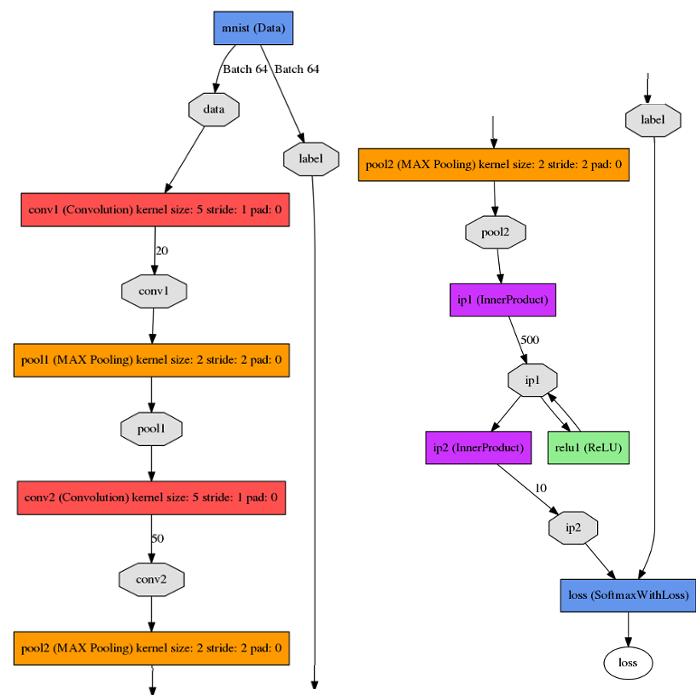
\includegraphics[width=0.8\textwidth]{figures/Original_net}
			\caption{Red básica LeNet \acrshort{mnist}.}
			\label{fig.redBasica}
		\end{center}
	\end{figure}
	
\subsubsection{Definición del solucionador}
	Para esta tarea se utiliza el archivo de Caffe \textit{lenet\_solver.prototxt}. En este documento se definen parámetros como la estructura de red que se utiliza, definida en el apartado anterior, y el número de iteraciones que se ejecutan durante el entrenamiento de la red, cuya explicación se aportó en la Sección~\ref{sec.caffe}. Además, en ese mismo capítulo, se explican el resto de parámetros que se manejan en este proyecto, como la evaluación de la red o las redes intermedias que se almacenan. A continuación se muestra el aspecto de este solucionador en Caffe, destacando los parámetros más significativos.
	\vspace{80pt}
	\begin{lstlisting}[frame=single]
	# The train/test net protocol buffer definition
	net: "examples/mnist/lenet_train_test.prototxt"
	# test_iter specifies how many forward passes the test should carry 
	# out.
	# In the case of MNIST, we have test batch size 100 and 100 test
	# iterations, covering the full 10,000 testing images.
	test_iter: 100
	# Carry out testing every 500 training iterations.
	test_interval: 500
	# The base learning rate, momentum and the weight decay of the network.
	base_lr: 0.01
	momentum: 0.9
	weight_decay: 0.0005
	# The learning rate policy
	lr_policy: "inv"
	gamma: 0.0001
	power: 0.75
	# Display every 100 iterations
	display: 100
	# The maximum number of iterations
	max_iter: 10000
	# snapshot intermediate results
	snapshot: 5000
	snapshot_prefix: "examples/mnist/lenet"
	# solver mode: CPU or GPU
	solver_mode: CPU	
	\end{lstlisting}
	
	Se debe fijar especial atención en parámetros como \textit{net}, que define la ruta al documento de la sección anterior en el que se define la estructura de red, \textit{test\_interval}, que marca cada cuántas iteraciones se realiza la evaluación de la red en el entrenamiento, \textit{max\_iter}, que define el número de iteraciones totales para finalizar el entrenamiento, \textit{snapshot}, que indica cada cúantas iteraciones se crea un archivo con la red intermedia correspondiente, y, finalmente, \textit{snapshot\_prefix}, que marca la ruta en la que se almacenan los archivos. La forma en la que se almacenan los archivos se corresponden con la ruta indicada hasta el último "\text{/}", siendo lo posterior el nombre deseado, completado con el número de iteración correspondiente. En el ejemplo mostrado, el archivo se almacena en la ruta \textit{"\text{examples/mnist/}"}    y el nombre de la red final es \textit{"lenet\_iter\_10000"}.\\
	
	Tras definir el solucionador se procede a la ejecución de un archivo que comience con el entrenamiento de la red y permita obtener, finalmente, el modelo entrenado para usar en la aplicación.
	
\subsubsection{Ejecución de la red}
	Para comenzar con el entrenamiento de la red, una vez definida la estructura y y el solucionador, se deben ejecutar los siguientes comandos:
	\vspace{10pt}
	\begin{lstlisting}[frame=single]
	cd $CAFFE_ROOT
	./examples/mnist/train_lenet.sh	
	\end{lstlisting}
	
	El archivo que se ejecuta contiene información sobre qué solucionador se debe implementar y el modo de ejecución, de la forma que se muestra a continuación.
	\vspace{10pt}
	\begin{lstlisting}[frame=single]
	#!/usr/bin/env sh
	set -e
	
	./build/tools/caffe train 
	  --solver=examples/mnist/lenet_solver_validation.prototxt 
	\end{lstlisting}
	
	Este archivo permite añadir una nueva línea mediante la que se obtiene, en la ruta marcada, un archivo de \textit{log} con información sobre el entrenamiento y la evaluación. Esta línea se añade tras indicar el solucionador de la forma que se muestra a continuación.
	\vspace{10pt}
	\begin{lstlisting}
	2>&1 | tee .../NombreArchivoLog.log $@
	\end{lstlisting} 
	
	En la Figura~\ref{fig.entrenamiento} se muestra la información que se observa en el terminal al ejecutar el entrenamiento, siendo ésta la misma que queda registrada en el archivo \textit{log} indicado.
	
	\begin{figure}[H]
		\begin{center}
			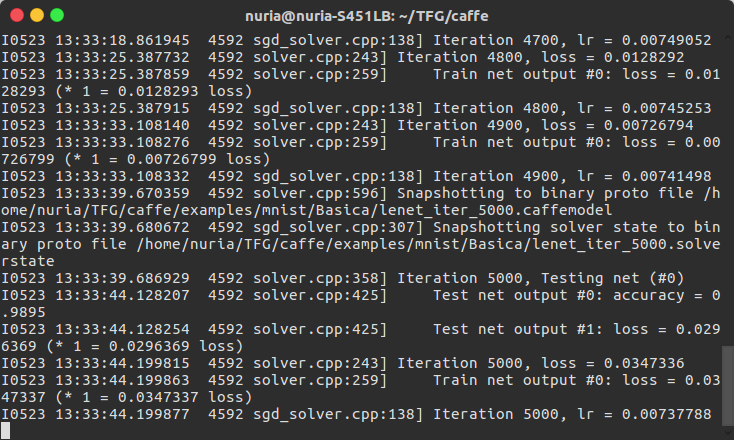
\includegraphics[width=0.8\textwidth]{figures/RedBasica5000}
			\caption{Ejecución de entrenamiento de red LeNet \acrshort{mnist}.}
			\label{fig.entrenamiento}
		\end{center}
	\end{figure}
	
	\begin{figure}[H]
		\begin{center}
			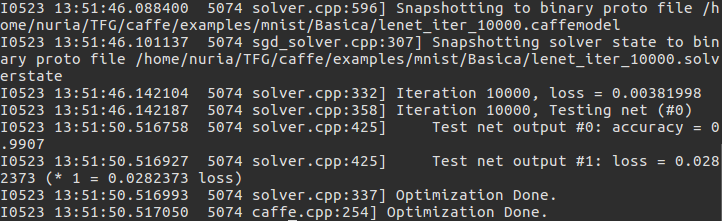
\includegraphics[width=0.8\textwidth]{figures/RedBasicaFin}
			\caption{Fin de entrenamiento de red LeNet \acrshort{mnist}.}
			\label{fig.finEntrBas}
		\end{center}
	\end{figure}
	
	Tras terminar el entrenamiento, mostrado en la Figura~\ref{fig.finEntrBas}, se obtiene el archivo con la red neuronal entrenada, almacenado según la ruta que se indicó en el solucionador, que podrá ser utilizada en la herramienta que sea de interés.\\

	Los parámetros de pérdidas y precisión calculados durante el entrenamiento para ambas fases quedan almacenados en el archivo \textit{log} generado, y son divididos en las dos fases, entrenamiento y evaluación, para su análisis. Para ello se ejecuta el archivo \textit{parse\_log.sh} proporcionado por la plataforma en su carpeta \textit{tools/extra}. En la Figura~\ref{fig.parse} se muestra el aspecto de estos archivos desglosados.
	\vspace{10pt}
	
	\begin{figure}[H]
			\centering
			\subfigure[]{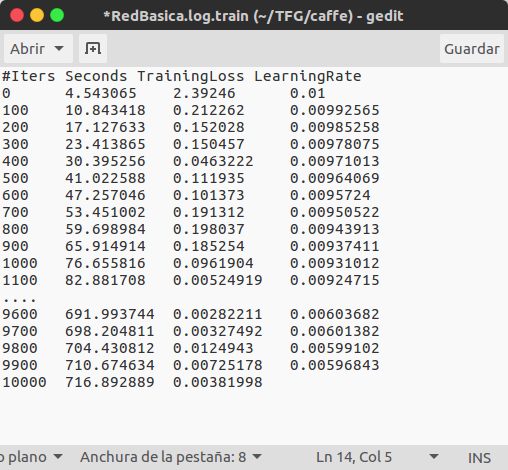
\includegraphics[width=0.45\textwidth]{figures/parselogtrain}}
			\subfigure[]{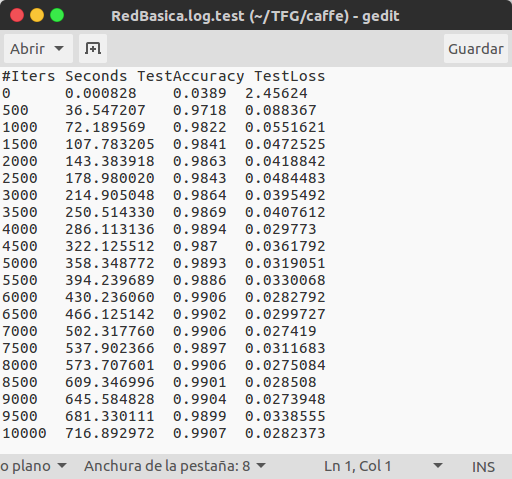
\includegraphics[width=0.45\textwidth]{figures/parselogtest}}
			\caption{Archivos \text{log} de: (a)~Entrenamiento, (b)~Evaluación.}
			\label{fig.parse}
	\end{figure}

\subsection{Componente clasificador} \label{sec.componente}
Se desarrolla un componente escrito en Python que, mediante la ayuda del \textit{Camera Server} de JdeRobot, comentado en la Sección~\ref{sec.jderobot},  y la red explicada en la Sección~\ref{sec.red}, es capaz de clasificar un dígito mostrado a la cámara, que se especifica en un archivo de configuración, en tiempo real, encendiendo una bombilla que se corresponde con el número obtenido. En la Figura~\ref{fig.componente} se muestra un diagrama de bloques con el diseño de este componente y todas sus entradas y salidas.\\
	
Debido a la magnitud de la tarea a realizar, se optó por dividir el programa en dos hilos que serán explicados a continuación. Uno de ellos se encargará del aspecto gráfico de la aplicación, mostrando la imagen obtenida por la cámara, la imagen procesada para la clasificación, y la iluminación de la bombilla correspondiente. El segundo hilo, se encargará de gestionar la captación de la cámara, mediante la conexión con el componente \textit{Camera Server}, así como el proceso de clasificación, utilizando la red entrenada. Todo el código correspondiente a esta aplicación se encuentra disponible en Github~\footnote{https://github.com/RoboticsURJC-students/2016-tfg-nuria-oyaga}.

\begin{figure}[H]
	\centering
	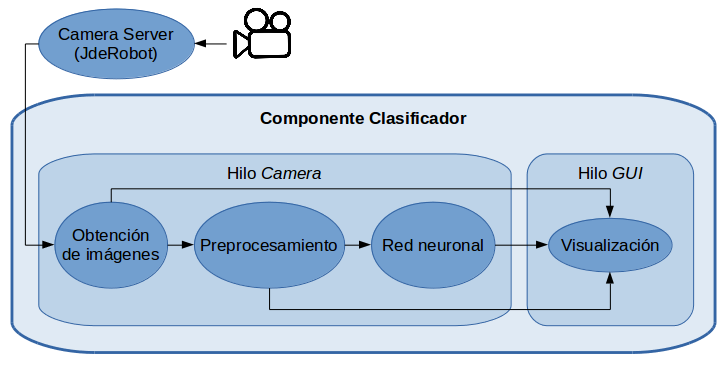
\includegraphics[width=0.8\textwidth]{figures/esquemaComponente}
	\caption{Esquema del componente.}
	\label{fig.componente}
\end{figure}

\subsubsection{Hilo \textit{Camera}} \label{sec.camara}
El hilo fundamental de la aplicación, que se encarga de la lógica de la misma mediante la adquisición de la imagen y su posterior procesamiento, está referenciado por el nombre \textit{Camera}.\\

Al comienzo de la ejecución se inicializa un objeto Cámara, mediante el constructor \textit{Camera()}, que será el encargado de gestionar las acciones anteriormente nombradas. En esta inicialización se indica qué cámara se va a utilizar, referenciada de manera externa mediante un archivo de configuración que se indica en la ejecución de la aplicación. La propiedad que indica la cámara en este archivo está enlazada con el componente \textit{Camera Server} de JdeRobot y es la siguiente:
\vspace{10pt}
\begin{lstlisting}[frame=single]
	Numberclassifier.Camera.Proxy=cameraA:default -h localhost -p 9999
\end{lstlisting}

Otro aspecto importante que se maneja en la inicialización de la cámara es la especificación y carga de la red que se empleará para la clasificación. Este aspecto se realiza mediante las siguientes líneas:
\vspace{10pt}
\begin{lstlisting}[frame=single]
	model_file = '.../lenet.prototxt'
	pretrained_file = '.../lenet_iter_10000.solverstate'
	self.net = caffe.Classifier(model_file, pretrained_file, 
									image_dims=(28, 28), raw_scale=255)
\end{lstlisting}

Con este código se realizan las tres acciones necesarias para establecer la red que se utiliza. En primer lugar, se indica cuál será el modelo empleado para la clasificación. Este modelo es un archivo porporcionado por Caffe de manera homóloga al \textit{lenet\_train\_test.prototxt}, con la excepción de que la capa de datos no recurre a archivos almacenados sino que utiliza imágenes que serán insertadas en la ejecución de la red. El resto de datos deben ser exáctamente iguales a la estructura de la red entrenada para que no se produzcan errores. En segundo lugar, se indica la red entrenada que se utiliza en la ejecución, el archivo obtenido al finalizar el entrenamiento según se indicó en la Sección~\ref{sec.red}. Por último, se crea la red ejecutable, es decir, se crea un objeto que será utilizado por la aplicación cada vez que se quiera realizar la clasificación. Para esta creación es necesario indicar, en primer lugar, que se trata de una red para la clasificación, y, además, introducir los parámetros del modelo, la red entrenada, las dimensiones de las imágenes, y la escala de los píxeles.\\

Además de las propiedades más importantes comentadas anteriormente, se definen también funciones que serán importantes para la ejecución de la aplicación. Se establece una función \textit{update(self)}, que será llamada cada 150ms para la actualización del hilo \textit{ThreadCamera(camera)}, creado en el componente principal, para obtener las imágenes de forma periódica y poder establecer un flujo de vídeo a tiempo real. Esta función, a su vez, necesita de otra, \textit{getImage(self)}, que obtiene la imagen, la redimensiona, y le aplica una transformación necesaria antes de introducirla en el proceso de clasificación, devolviendo un array con las dos imágenes, original y transformada. Para esa transformación se utiliza una tercera función de la cámara, \textit{trasformImage(self,img)}. En ella, se centra la imagen en un cuadrado, pues la captada es rectangular y la necesaria para introducir en la red debe ser cuadrada, se convierte a imagen de grises, se redimensiona al tamaño necesario para introducirla en la red (28x28), se le aplica un filtro gaussiano de 5x5 para reducir el ruido,y por último, se aplica un filtro de transformación por gradiente para lograr independencia de los niveles de intensidad particulares en las imágenes.\\

Finalmente, se crea una función para realizar la clasificación de los dígitos.En primer lugar se asegura que las dimensiones del \textit{blob} de datos sea de 28x28. En el siguiente paso, se introduce a la red la imagen obtenida tras la transformación, aplicandole el factor de escala para que el intervalo de los píxeles esté entre 0 y 1, coincidiendo con el aprendizaje. Posteriormente se ejecuta la red y se obtiene, como salida, una estructura que almacena, por un lado, la propiedad \textit{'prob'} que se corresponde con un array que incluye las probabilidades de que la imagen introducida sea cada uno de los dígitos posibles, y, por otro, el tipo de datos que se almacena, en este caso \textit{float32}. Posteriormente, de ese array de probabilidades, se escoge el dígito cuya probabilidad es mayor y se devuelve. Todo ello queda implementado con el siguiente código:
\vspace{10pt}
\begin{lstlisting}[frame=single]
	def classification(self, img):
		self.net.blobs['data'].reshape(1,1,28,28)
		self.net.blobs['data'].data[...]=img * 0.00390625
		output = self.net.forward()
		digito = output['prob'].argmax()
		return digito
\end{lstlisting}

Una vez establecida la lógica de la aplicación, se procede a desarrollar el interfaz gráfico que permite al usuario visualizar, tanto las imágenes captadas y transformadas, como el resultado de la clasificación.

\subsubsection{Hilo de interfaz gŕafico}
Para el aspecto gráfico de la aplicación, en el componente principal se inicializa un objeto llamado \textit{window} mediante el constructor \textit{Gui()}, al que posteriormente se le vincula la cámara mediante una función propia, \textit{window.setCamera(camera)}. Por último, al tratarse de un componente gráfico, es necesario indicar que se muestre mediante \textit{window.show()}. Al inicializar este objeto se crean todos los elementos gráficos que son necesarios y que se modificarán posteriormente para conseguir el resultado deseado.\\

Al igual que en el caso de la cámara, se establece un hilo que permite aligerar la ejecución de la aplicación mediante \textit{ThreadGui(window)}, que establece el tiempo de actualización en 50ms. Debido al uso de este hilo, se crea en el objeto una función \textit{update()} que, en este caso, se encarga de obtener las imágenes original y transformada mediante la función \textit{getImage()} de la cámara, y adaptarlas para poder mostrarlas en las etiquetas definidas para cada una de ellas. Además, llama a otra función propia, \textit{lightON(out)}, que cambia el color del fondo del dígito que se haya clasificado, haciendo uso de la función de clasificación definida anteriormente en la cámara.\\

En la Figura~\ref{fig.gui} se puede observar el resultado gráfico de la aplicación. Al no tener detección, la ejecución de la clasificación es continua, por lo que, aunque no exista un dígito en la imagen, el componente decide constantemente un determinado dígito que considera correcto, encendiendo la bombilla adecuada.

\begin{figure}[H]
	\begin{center}
		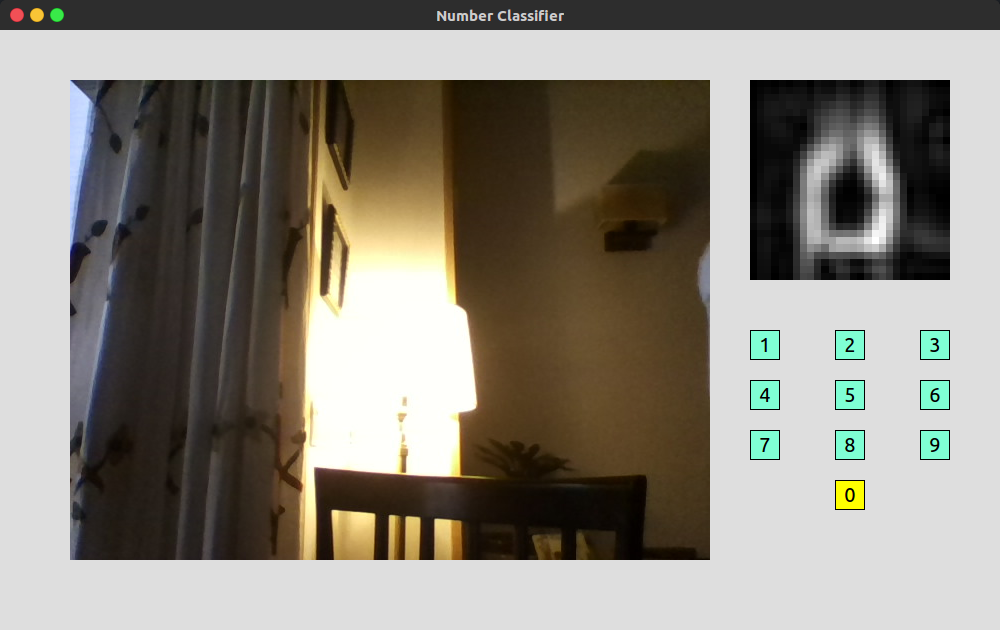
\includegraphics[width=0.65\textwidth]{figures/gui}
		\caption{Captura de componente gráfico de la aplicación.}
		\label{fig.gui}
	\end{center}
\end{figure}

\subsubsection{Ejecución del componente}
El proceso de ejecución del componente se divide en dos pasos. Por un lado, es necesaria la ejecución del servidor de imágenes, para lo que se utiliza el componente de JdeRobot. Por otro lado se debe lanzar el propio componente clasificador explicado anteriormente.\\

Para ejecutar el \textit{Camera Server}, se siguen las instrucciones que aporta la plataforma JdeRobot, utilizando el archivo de configuración que se facilita. Se utiliza el siguiente comando: 
\vspace{10pt}
\begin{lstlisting}[frame=single]
	cameraserver cameraserver.cfg
\end{lstlisting}

En este trabajo, la propiedad de interés del archivo de configuración es \textit{Camera.0.Uri}, que indica la fuente de vídeo. Esta fuente puede ser un archivo de vídeo almacenado, para el que se emplea la ruta del archivo en ese campo, la webcam del propio ordenador, para el que se utiliza el valor 0, u otra cámara externa, para la que se le indica el valor 1.\\

En la Sección~\ref{sec.droid} se comentó una aplicación que permite utilizar la camara de un smartphone android como fuente de vídeo mediante una cámara externa. Para poder utilizar esta herramienta es necesario tener instalados el programa tanto en el dispositivo móvil a utilizar como en el propio ordenador, según se indica en la guía de la aplicación~\footnote{https://www.dev47apps.com/droidcam/linuxx/}, y abrir la aplicación. Una vez abierta en ambos dispositivos, se debe conectar el USB del ordenador al móvil e indicar en la aplicación de escritorio que la conexión se hará vía USB. La razón del uso del USB y no de la conexión vía \textit{WiFi} radica en la rapidez, siendo más adecuada para tiempo real. Una vez se han realizado las acciones anteriores se estable la conexión y se obtienen los resultados de la Figura~\ref{fig.droid} para el ordenador y el dispositivo.\\

\begin{figure}[H]
	\centering
	\subfigure[]{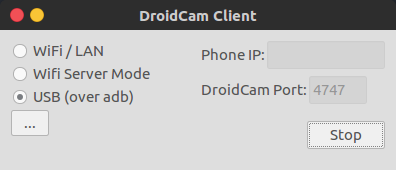
\includegraphics[width=0.4\textwidth]{figures/droidcamEscr}} \hspace{10pt}
	\subfigure[]{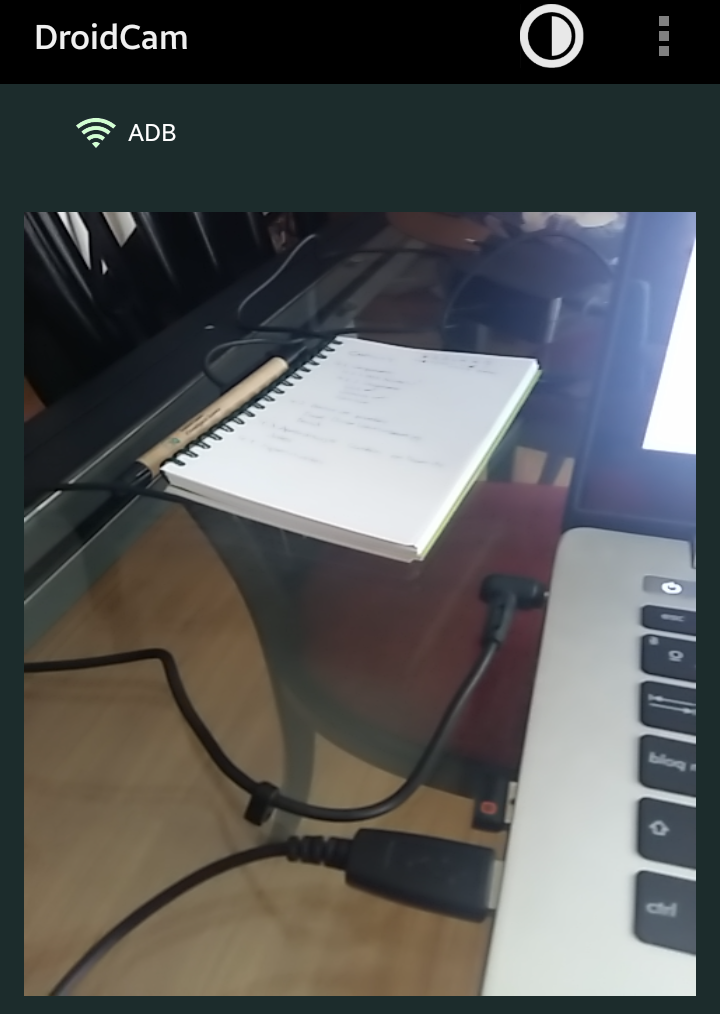
\includegraphics[width=0.3\textwidth]{figures/droidcamMov}}
	\caption{Capturas de DroidCam en: (a)~Escritorio, (b)~Dispositivo móvil}
	\label{fig.droid}
\end{figure}

Al incluir esta aplicación, el esquema de las conexiones del componente se modifica, dando lugar a una nueva estructura mostrada en la Figura~\ref{fig.esquemaDroid}

\begin{figure}[H]
	\centering
	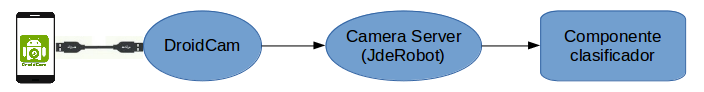
\includegraphics[width=0.8\textwidth]{figures/esquemaDroid}
	\caption{Esquema de conexión con DroidCam.}
	\label{fig.esquemaDroid}
\end{figure}
\vspace{20pt}

Tras tener en funcionamiento el servidor de imágenes se procede a la ejecución del componente clasificador, para ello se ejecuta el siguiente comando:
\vspace{10pt}
\begin{lstlisting}[frame=single]
	python numberclassifier.py --Ice.Config=numberclassifier.cfg
\end{lstlisting}

El componente Python contiene los procedimientos indicados en las secciones anteriores, la creación del GUI, la cámara y el lanzamiento de los hilos correspondiente a cada uno de ellos. En el fichero de configuración se tiene una propiedad que indica qué cámara utilizar, es importante que el nombre de esta cámara se corresponda con el indicado en el fichero de configuración del servidor, de esta manera se establece la comunicación entre ambos componentes.\\

Finalmente, tras la ejecución, obtenemos el resultado del componente mostrado en la Figura~\ref{fig.componente1}, donde se aprecia el funcionamiento del mismo para un número sencillo.

\begin{figure}[H]
	\begin{center}
		\subfigure[]{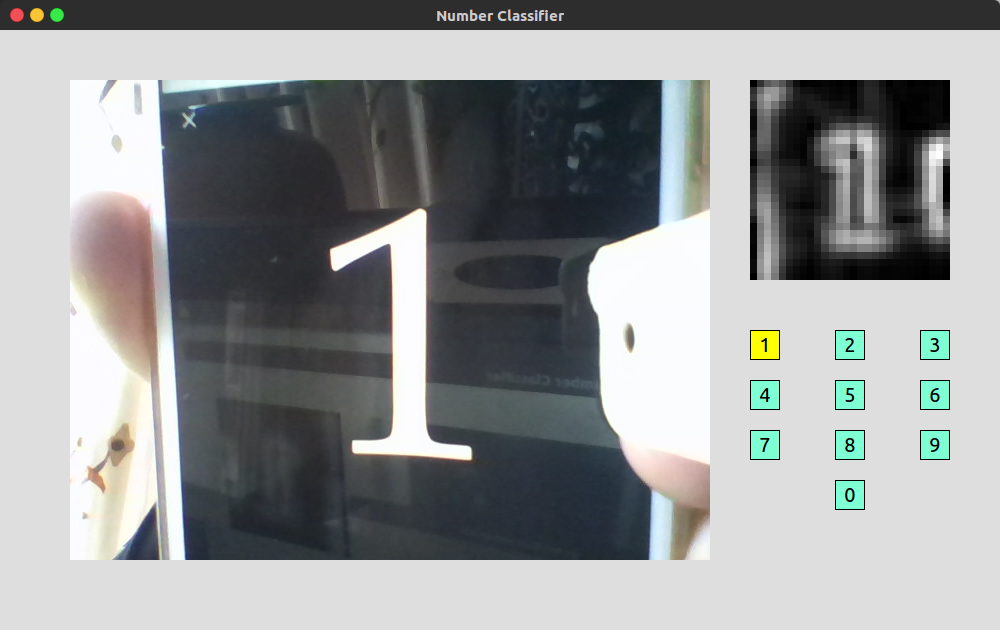
\includegraphics[width=0.4\textwidth]{figures/fondoNegro}}\hspace{10pt}
		\subfigure[]{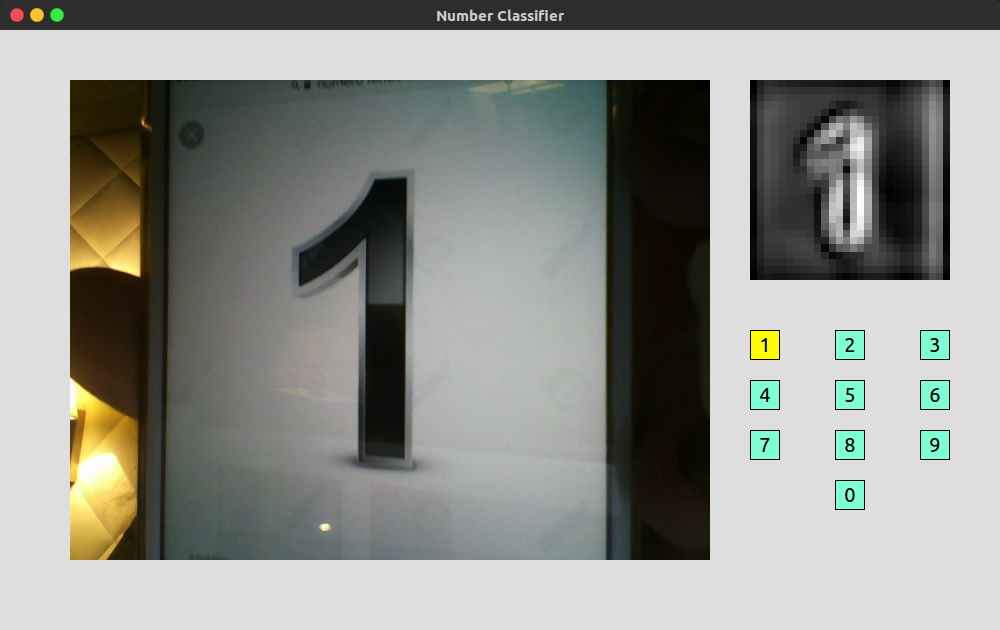
\includegraphics[width=0.4\textwidth]{figures/fondoBlanco}}
		\caption{Ejemplo del componente clasificador con: (a)~Fondo negro, (b)~Fondo blanco.}
		\label{fig.componente1}
	\end{center}
\end{figure}

Tras conseguir la aplicación del clasificador, se ha evaluado la red obtenida mediante un banco de pruebas, que será explicado a continuación y se ha procedido a la mejora de la misma gracias a los diferentes resultados obtenidos.

\section{Banco de pruebas} \label{sec.banco}
Para evaluar las redes neuronales que se desarrollan en el proyecto se elabora un banco de pruebas que permite obtener las medidas de prestaciones explicadas en el Capítulo~\ref{cap.infraestructura}, a partir de una base de datos de test.

\subsection{Obtención de datos de test}
El primer paso para elaborar este banco de pruebas pasa por el desarrollo de un \textit{script}, \textit{testcaffenet.py}, que permite introducir una base de datos de test a la red neuronal y obtener la clasificación para cada elemento. Este \textit{script} está dividido en tres partes claramente diferenciadas que permite la obtención de los resultados finales y que serán detalladas a continuación.

\begin{description}
	\item[Obtención de las imágenes] \hfill 
	\vspace{5pt}
	\\
	Las imágenes y las etiquetas que las identifican en una determinada clase estan almacenadas en bases de datos de tipo \textit{\acrfull{lmdb}}. Este tipo de bases de datos requieren de un método específico para acceder a su contenido y poder manipular las imágenes que se almacenan en ellas, que queda definido a continuación.
	\vspace{10pt}
	\begin{lstlisting}[frame=single]
	lmdb_env = lmdb.open('.../test_lmdb')
	lmdb_txn = lmdb_env.begin()
	lmdb_cursor = lmdb_txn.cursor()
	\end{lstlisting}
	
	Tras este código se obtiene un puntero que apunta al comienzo de los datos en la base de datos y que permitirá recorrerla para obtener las imágenes y sus etiquetas.\\
	\vspace{-10pt}
	\\
	Para procesar los datos obtenidos anteriormente utilizando la plataforma Caffe, será necesario crearse una estructura \textit{Datum} de la propia plataforma. Esta estructura incluye, en cada iteración para recorrer la base de datos, la información de la instancia que se analiza. El siguiente código crea la estructura indicada e indica la forma en que se recorre la base de datos, obteniendo, por un lado, los datos de la imagen en sí (\textit{data}), y por otro, sus etiquetas (\textit{label}).
	\vspace{10pt}
	\begin{lstlisting}[frame=single]
	datum = caffe.proto.caffe_pb2.Datum()
	...
	for key, value in lmdb_cursor:
		datum.ParseFromString(value)
		label = datum.label
		data = caffe.io.datum_to_array(datum)
		...
	\end{lstlisting}
	
	Finalmente, en la variable \textit{data} se almacena la imagen que se utilizará posteriormente para realizar la clasificación, y en \textit{label} la etiqueta correspondiente que se empleará para evaluar la capacidad de generalización de la red.
	\vspace{5pt}
	\item[Clasificación de las imágenes] \hfill 
	\vspace{5pt}
	\\
	La tarea de clasificación se realizará de la misma manera que se especificó en la Sección~\ref{sec.camara}, utilizando la misma función sobre cada uno de los \textit{data} obtenidos, según se muestra en el código a continuación.
	\vspace{25pt}
	\begin{lstlisting}[frame=single]
	...
	net_out = classification(data)
	...
	\end{lstlisting}
	
	Una vez obtenido el dígito que la red interpreta, se procede a comparar éste con la etiqueta verdadera para evaluar las prestaciones de la red.
	\vspace{5pt}
	\item[Evaluación de prestaciones] \hfill 
	\vspace{5pt}
	\\
	Para obtener resultados que puedan ser procesados por el banco de pruebas se creará un archivo de texto con la información necesaria. En este archivo se incluye una descripción del contenido y, para cada muestra procesada por la red, su número, la etiqueta real, la identificada por el clasificador y un booleano que indicará la coincidencia entra ambas. La obtención de este archivo de texto se logra gracias al siguiente código:
	\vspace{10pt}
	\begin{lstlisting}[frame=single]
	for key, value in lmdb_cursor:
		...
		if label == net_out:
			conclusion = True
		else:
			conclusion = False
		testfile.write("Interacion " + str(loop) + ":")
		testfile.write(str(label) + " " + str(net_out) + " " )
		testfile.write(str(conclusion) + "\n")
		...
	\end{lstlisting}
	
	Esta estructura permitirá un manejo más cómodo de los resultados por el banco de pruebas creado, además de una mejor comprensión para el usuario que lea el archivo.
\end{description}

\subsection{Banco de pruebas manual}
Las medidas de prestaciones que se obtienen con este banco de pruebas son los explicados en la Sección~\ref{sec.prestaciones}: Matriz de confusión, \textit{precision} y \textit{recall}. De manera externa al banco de pruebas, y gracias a Caffe, se obtendrán también valores de \textit{accuracy}, homólogo a la tasa de acierto, y \textit{loss}, para cada una de las redes intermedias que se obtienen durante el entrenamiento hasta alcanzar la red final, y la propia red.\\

Para la elaboración de este banco de pruebas se ha optado por la herramienta de \textit{Libre Office Calc}, que permite realizar diversas operaciones sobre hojas de cálculo gracias a múltiples fórmulas y funciones. Se han volcado los datos obtenidos con el \textit{script} anterior estableciendo como separador el espacio y los dos puntos, obteniendo así distintas columnas, cada una de ellas con un determinado dato. De estas columnas, serán de interés la que contiene la etiqueta real, la clasificación realizada, y la conclusión final, acierto o fallo.\\

Una vez se dispone de los datos necesarios para la evaluación de prestaciones, separados y correctamente ordenados, se procederá a identificar el número de aciertos y fallos obtenidos. Esta acción es llevada a cabo a nivel global, para obtener los parámetros de tasa de acierto o \textit{accuracy}, y a nivel de dígito, para obtener la matriz de confusión y con ella los valores de \textit{precision} y \textit{recall} para cada uno de los dígitos.

\begin{description}
	\item[Tasa de acierto] \hfill 
	\vspace{5pt}
	\\
	Este valor es el más sencillo de obtener. Para calcular la tasa de acierto, independientemente del dígito que se trate, basta con contar el número de veces que se ha obtenido el valor \textit{True} en la columna de conclusión y dividirlo entre el número de imágenes de test. De esta manera se obtiene el porcentaje de imágenes que se han clasificado de forma correcta, valor que se corresponde con una estimación de la tasa de acierto de la red.\\
	\vspace{-10pt}
	\\
	Para calcular la tasa de acierto, el código empleado ha sido dividido en cuatro partes diferenciadas, obteniendo en cada una de ellas uno de los valores para obtener el resultado final, que serán expuestas a continuación.\\
	\vspace{10pt}
	\begin{itemize}
		\item{Para obtener el número de clasificaciones correctas:
		\vspace{10pt}
		\begin{lstlisting}[frame=single]
	CONTAR.SI('Sobel sin trasform'.E3:E20002;"True")
		\end{lstlisting}
		Donde:
		\begin{itemize}
			\item `Sobel sin transform' es la hoja en la que se han volcado los resultados del archivo de texto.
			\item E3:E20002 es la columna que contiene los datos de la conclusión.
			\item ``True'' indica que se quiere contar el número de veces en esa columna que aparece ese valor
		\end{itemize}
	}
	\item{Para obtener el número de clasificaciones incorrectas:
		\vspace{10pt}
		\begin{lstlisting}[frame=single]
	CONTAR.SI('Sobel sin trasform'.E3:E20002;"False")
		\end{lstlisting}
		Es equivalente al anterior pero, en este caso, se cuenta el número de veces que se cometió un error en la clasificación.
	}
	\item{Para obtener el número de imágenes de evaluación totales será suficiente con realizar la suma de los correctos e incorrectos.
	}
	\item{Para calcular el porcentaje de acierto se realizará la división del número de aciertos entre el total y se multiplicará por 100 para obtener el porcentaje.
	}
	\end{itemize}
	\vspace{5pt}
	\item[Matriz de confusión] \hfill 
	\vspace{5pt}
	\\
	Para elaborar la matriz de confusión se parte de la misma hoja de cálculo del apartado anterior. En este caso, para cada dígito real, se debe tener en cuenta tanto el número de veces que se clasifica correctamente, como el número de veces que se equivoca con cada uno de los dígitos restantes.\\
	\vspace{-10pt}
	\\
	Se elabrora una tabla en la que se enfrentan los dígitos reales, del 0 al 9, con las predicciones. En concreto, cada columna representa las veces que se presenta cada uno de los dígitos y, cada fila el número de veces que éste se predice.\\
	\vspace{-10pt}
	\\
	El código de cada celda queda materializado de la siguiente manera:
	\vspace{10pt}
	\begin{lstlisting}[frame=single]
	CONTAR.SI.CONJUNTO(C3:C70002;"1";D3:D70002;"2")
	\end{lstlisting}
	Donde:
	\begin{itemize}
		\item C3:CC70002 se corresponde con la columna que contiene las etiquetas reales
		\item D3:D70002 se corresponde con la columna que contiene las etiquetas predichas.
		\item Los valores entre comillas, ``1'' y ``2'' se corresponde con el dígito que se quiera analizar, siendo el primer valor el real y el segundo el predicho. En este caso, se está contando el número de veces que se ha producido un 1 y se ha predicho, erróneamente, un 2.
	\end{itemize}
	
	De esta forma, cada vez que se prediga un dígito determinado, se sumará una unidad en la celda que se corresponda con el dígito real introducido en la red y la etiqueta ofrecida por la red. Una vez se dispone de esta matriz, obtener los valores de \textit{precision} y \textit{recall} resulta bastante sencillo.
	\vspace{5pt}
	\item[\textit{Precision}] \hfill 
	\vspace{5pt}
	\\
	Para obtener el valor de \textit{precision} para cada dígito, se divide el número de veces que se ha clasificado correctamente dicho dígito entre el número de veces totales que se predijo el mismo. Para ello, se suman todos los valores por filas, obteniendo el número de predicciones de cada uno de los dígitos, y se divide cada valor de la diagonal, correspondiente con las clasificaciones correctas, entre el valor suma obtenido en la fila correspondiente.
	\vspace{5pt}
	\item[\textit{Recall}] \hfill 
	\vspace{5pt}
	\\
	Para este parámetro, se debe dividir el número de clasificaciones correctas de cada dígito entre el número de veces que se produjo el mismo. En este caso, se sumarán los valores obtenidos por columnas, lo que dará por resultado el número de veces que se introdujo a la red cada uno de los dígitos. Una vez obtenido ese valor, se debe dividir el valor de la diagonal correspondiente, al igual que en el caso anterior, entre el valor obtenido para cada columna.
\end{description}
\vspace{10pt}
\section{Efectos del aprendizaje} \label{sec.aprendizaje}
Existen numerosos factores que afectan a la robusted del diseño. Elementos como la base de datos, el número de neuronas empleadas, el número de capas o etapas en el entrenamiento~\cite{lopez2008redes}, influyen en la robusted de la red.\\

En esta sección se tratará el efecto que la base de datos de entrenamiento/validación y el número de iteraciones tienen en las prestaciones de la red.

\subsection{Aprendizaje con imágenes originales}
La base de datos empleada en el primer ejemplo es excesivamente simple y, por lo tanto, no aporta la robusted necesaria para un problema de clasificación real. Por ello se estudiará la ampliación y modificación de la misma para obtener una red robusta que permita la clasificación de imágenes reales de la manera más precisa posible.\\

Una particularidad de la base de datos de \acrshort{mnist} es que únicamente dispone de ejemplos con el fondo negro y el dígito en blanco. Esto limita bastante la funcionalidad de la aplicación, ya que se pretende clasificar dígitos independientemente del fondo sobre el que éstos se muestren. Para estudiar el efecto que tiene el cambio de fondo en las imágenes, se ha ampliado la base de datos incluyendo, para cada muestra, su negativo. La nueva base de datos se consigue gracias al \textit{script} \textit{create\_neg\_database.py}, que parte del tratamiento de bases de datos de tipo \acrshort{lmdb} explicado en la Sección~\ref{sec.banco}. Se debe abrir la base de datos con las imágenes originales y realizar la transformación deseada. Posteriormente, para almacenar las imágenes transformadas, se debe abrir una nueva base de datos de este tipo que permita escritura, según se muestra a continuación.
\vspace{10pt}
\begin{lstlisting}[frame=single]
	new_lmdb_env = lmdb.open('.../database_lmdb', map_size=int(1e12))
	new_lmdb_txn = new_lmdb_env.begin(write=True)
	new_lmdb_cursor = new_lmdb_txn.cursor()
	new_datum = caffe.proto.caffe_pb2.Datum()
	\end{lstlisting}

Se puede observar que el proceso es muy similar al explicado en la Sección~\ref{sec.banco}, incluyendo dos parámetros que permitan la escritura en la base de datos. Posteriormente, dentro del bucle, se debe almacenar la imagen original en la nueva base de datos, aplicar el negativo, y almacenar, también, el resultado de la transformación.\\

Para insertar imágenes en una nueva base de datos es necesario realizar dos acciones, la inserción en la base de datos y su actualización:
\vspace{10pt}
\begin{lstlisting}[frame=single]
	new_datum = caffe.io.array_to_datum(data,label)
	keystr = '{:0>8d}'.format(item_id)
	new_lmdb_txn.put( keystr, new_datum.SerializeToString() )
\end{lstlisting}

De esta manera se incluye en la posición \textit{keystr}, la imagen y la etiqueta deseada, a partir del puntero que señala las posiciones dentro de la base de datos. Posteriormente, para la actualización de la base de datos, se debe incluir un nuevo código que guarda los cambios realizados y actualiza la posición del puntero.
\vspace{10pt}
\begin{lstlisting}[frame=single]
	new_lmdb_txn.commit()
	new_lmdb_txn = new_lmdb_env.begin(write=True)
\end{lstlisting}

Las anteriores líneas se incluyen dentro de un condicional que hará que únicamente se escriba en la base de datos cada cierto tiempo, ya que no es necesario realizar estas acciones en todas las inserciones realizadas, ahorrando carga computacional.\\
\vspace{20pt}

En la Figura~\ref{fig.neg} se muestra el negativo almacenado en la base de datos para cada dígito mostrado en la Figura~\ref{fig.digitosMNIST}. Estas imágenes han sido obtenidas con el \textit{script} \textit{dataread.py}, que lee las imágenes de la base de datos y crea un archivo para su visualización.\\

\begin{figure}[H]
	\begin{center}
		
\includegraphics[width=0.3\textwidth]{figures/negativo}
		\caption{Negativo de muestras de la base de datos.}
		\label{fig.neg}
	\end{center}
\end{figure}

Tras ejecutar el \textit{script} que aumenta la base de datos con la transformación, se obtiene una nueva base de datos de test con los negativos, la cual tendrá el doble de muestras que en el caso original, es decir 20000 ejemplos. Ésta es introducida en el banco de pruebas y a partir de ella se obtienen valores de tasa de acierto.\\

En la Figura~\ref{fig.neg-orig} se muestran los resultados obtenidos tras entrenar la red con el conjunto de entrenamiento  de \acrshort{mnist}, tras la división entrenamiento/validación, y evaluada con las bases de datos de test \textit{mnist} y aumentada con el negativo. Obsérvese que la red falla considerablemente al incluir las imágenes en negativo.

\begin{figure}[H]
	\begin{center}
		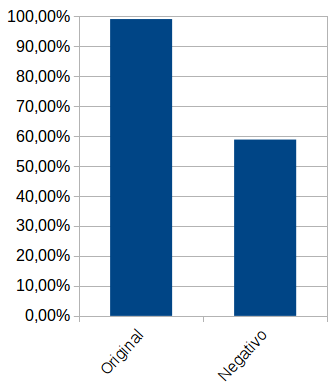
\includegraphics[width=0.4\textwidth]{figures/orig_neg}
		\caption{Porcentaje de acierto sobre red entrenada con \acrshort{mnist} y evaluada con base de datos original y ampliada con negativo.}
		\label{fig.neg-orig}
	\end{center}
\end{figure}

\subsection{Aprendizaje con transformación por gradiente}
\label{sec.bordes}
Para mejorar la capacidad de generalización de la red, puesto que la aplicación no está enfocada a un único tipo de fondo, se opta por aplicar un filtro de gradiente que independice la representación del contenido de la imagen de los niveles de intensidad. Existen varios filtros de gradiente~\cite{fundamentos}.\\

Para desarrollar la comparación entre los diferentes filtros se ha desarrollado un \textit{script} similar al anterior, en el que se aplicaba el negativo, \textit{create\_edges\_database.py}, que aplicará el filtro de borde seleccionado. Se parte de la base de datos ampliada con el negativo, por lo que no es necesario almacenar la imagen de la que se parte en la base de datos. Será necesario aplicar el filtro también sobre los ejemplos de entrenamiento y validación, puesto que el objetivo es desarrollar una nueva red neuronal que interprete los bordes. Se obtiene, así, una base de datos de entrenamiento con 48000 muestras, otra de validación con 12000, y una última de test con 20000, a las que se les ha aplicado un determinado filtro de bordes. A continuación se explicarán los tres filtros evaluados en este proyecto: Canny, Laplaciano y Sobel.
\vspace{10pt}
\begin{description}
	\item[Filtro de Canny] \hfill 
	\vspace{5pt}
	\\
	El algoritmo de Canny es un operador desarrollado por John F. Canny en 1986 que utiliza un algoritmo de múltiples etapas para detectar una amplia gama de bordes en imágenes~\cite{4767851}. Para ello utiliza el cálculo de variaciones, una técnica que encuentra la función que optimiza un funcional indicado. En este caso, la función óptima es definida por la suma de cuatro términos exponenciales, pero se puede aproximar por la primera derivada de una gaussiana. El resultado de aplicar este filtro es siempre una imagen binaria en la que los píxeles únicamente pueden tomar los valores 0 ó 1 (0 ó 255 dependiendo del rango).\\
	\vspace{-10pt}
	\\
	Para aplicar este algoritmo en el código se debe implementar la función proporcionada por \textit{openCV}~\cite{cannyOCV}. En la base de datos de test se obtienen dos imágenes iguales de cada dígito, ya que el mismo filtro se está aplicando sobre el original y el negativo el mismo filtro.
	\vspace{20pt}
	\item[Filtro Laplaciano] \hfill 
	\vspace{5pt}
	\\
	El laplaciano es un operador de segunda derivada que se utiliza con frecuencia en la detección de bordes~\cite{laplacian}~\cite{gonzalez2008digital}, identificando un borde cuando se produce un cruce por cero en la segunda derivada. Este operador posee dos filtros diferentes, uno positivo con el que se obtienen los bordes y uno negativo. Estos filtros proporcionan resultados diferentes ya que al aplicar el filtro positivo únicamente se tienen en cuenta los cruces por cero crecientes en la segunda derivada, mientras que en el negativo se consideran los decrecientes. Este hecho da lugar a la obtención de dos tipos de borde: el externo en el positivo, utilizado en este trabajo, y el interno en el negatovo. El resultado final será una imagen en escala de grises correspondiente con los bordes de interés.\\
	\vspace{-10pt}
	\\
	La aplicación del filtro es posible gracias a otra función de \textit{openCV}~\cite{laplacianOCV}. Al aplicar este filtro sobre las imágenes originales y su negativo no se obtiene exactamente la misma imagen. Al aplicar el filtro positivo sobre la imagen original, con el fondo negro, se obtienen los bordes externos de la misma, sin embargo, al invertir los niveles de intensidad, la derivada de la imagen se invierte de la misma manera. Este hecho hace que lo que se considera como bordes externos en la imagen de negativo se corresponda con lo que eran bordes internos en la original. Esta diferencia podría perjudicar a la robustez de la red, pues dependiendo de la imagen la diferencia entre ambos podría ser suficiente como para crear confusión.
	\vspace{10pt}
	\item[Filtro de Sobel] \hfill 
	\vspace{5pt}
	\\
	Este filtro está formado por dos máscaras que permiten obtener una aproximación a la derivada en las direcciones horizontal y vertical~\cite{gonzalez2008digital}. Para obtener la imagen de bordes final será necesario sumar ambas soluciones, en valor absoluto, obteniendo la imagen de grises con los bordes.\\
	\vspace{-10pt}
	\\
	Para aplicar este filtro, primero se debe aplicar cada una de las dos máscaras, horizontal y vertical, gracias a la función de \textit{openCV}~\cite{sobelOCV}. Una vez se tienen los bordes en ambas direcciones, se suman sus valores absolutos y se normaliza a valores entre 0 y 255, obteniendo una imagen de tipo \textit{float} que deberá ser transformada a \textit{uint8}. En este caso, y al igual que en el caso de Canny, se obtiene la misma imagen de bordes en ambas imágenes, pues el filtro no hace distinción entre bordes internos y externos.	
\end{description}

\begin{figure}[H]
	\centering
	\subfigure[]{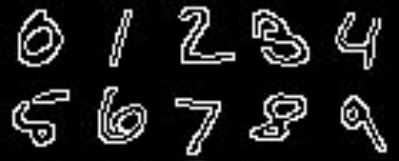
\includegraphics[width=0.4\textwidth]{figures/canny}} \hspace{10pt}
	\subfigure[]{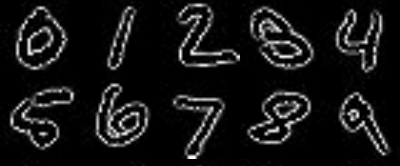
\includegraphics[width=0.4\textwidth]{figures/laplacian-orig}} \hspace{10pt}
	\subfigure[]{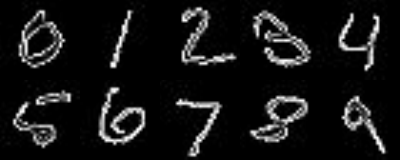
\includegraphics[width=0.4\textwidth]{figures/laplacian-neg}} \hspace{10pt}
	\subfigure[]{
\includegraphics[width=0.4\textwidth]{figures/sobel}}
	\caption{Muestras de imágenes de bordes: (a)~Canny, (b)~Laplaciano sobre original, (c)~Laplaciano sobre negativo, (d)~Sobel.}
	\label{fig.bordes}
\end{figure}
\vspace{20pt}

La Figura~\ref{fig.bordes} muestra la aplicación de las tres transformaciones por gradiente explicadas para cada dígito mostrado en la Figura~\ref{fig.digitosMNIST}, incluyendo las dos versiones del filtro Laplaciano, los bordes obtenidos para la original y su negativo.\\

Una vez obtenidas las diferentes bases de datos, con los filtros de bordes aplicados, se procede al entrenamiento de tres redes neuronales diferentes. Cada red se entrena con uno de los filtros, según se explicó en la Sección~\ref{sec.red}, modificando únicamente las bases de datos empleadas en entrenamiento y evaluación.\\

Tras entrenar las tres redes neuronales será posible comenzar con el test de las mismas, obteniendo la tasa de acierto representadas en la Figura~\ref{fig.filtros}. Para ello se ha empleado la base de datos de test ampliada con el negativo aplicando, para cada red, el filtro correspondiente.

\begin{figure}[H]
	\begin{center}
		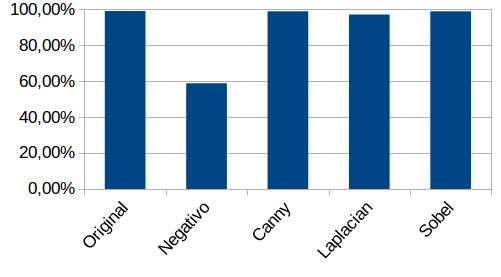
\includegraphics[width=0.5\textwidth]{figures/filtros}
		\caption{Comparación de tasa de acierto para la red entrenada con el conjunto original y evaluada con base de datos de test original y ampliado con negativo, y redes entrenadas con la base de datos con el filtro indicado y evaluada con la de test del mismo filtro.}
		\label{fig.filtros}
	\end{center}
\end{figure}

En la Figura~\ref{fig.filtros} se puede observar que el uso de imágenes de bordes mejora en gran medida el entrenamiento, haciendo la clasificación independiente de los niveles de intensidad particulares. Los filtros utilizados producen prácticamente el mismo resultado, siendo ligeramente peor el filtro laplaciano por la diferencia entre bordes internos y externos explicada anteriormente. Por todo ello, y por la preferencia de obtener imágenes en tono de grises que hagan más robusta la red, se elige el filtro de Sobel en la aplicación.\\

\subsection{Otras transformaciones. \textit{Data Augmentation}}
Al obtener una imagen con la cámara, ésta puede no estar perfectamente centrada, estar girada o a una escala diferente al de la base de datos empleada en el entrenamiento. Además, puede incluir ruido introducido por la propia cámara. Esto hará que, si la red ha sido entrenada con imágenes sin ningún tipo de alteración, ésta no generalice bien.\\

A continuación se explicarán las distinas transformaciones que serán aplicadas, todas ellas con ayuda de las funciones que proporciona \textit{openCV}.
\vspace{10pt}
\begin{description}
	\item[Rotación] \hfill 
	\vspace{5pt}
	\\
	La rotación consiste en el giro un determinado ángulo sobre un eje situado en el centro de la imagen. En concreto, en esta aplicación se ha optado por la rotación con un ángulo aleatorio en el rango [-20,20] grados.
	\vspace{10pt}
	\item[Traslación] \hfill 
	\vspace{5pt}
	\\
	La traslación de una imagen consiste en desplazar la misma según un determinado vector definido por dos variables \textit{x} e \textit{y}, tomando como referencia el eje central.\\
	\vspace{-10pt}
	\\
	Para la evaluación que es de interés en el proyecto, se ha establecido un rango de desplazamiento horizontal aleatorio de [-4,4] píxeles y uno vertical de [-4,2] píxeles, de tal manera que la imagen del dígito no quede recortada.
	\vspace{10pt}
	\item[Escalado] \hfill 
	\vspace{5pt}
	\\
	El escalado de una imagen consiste en cambiar la escala de la misma estableciendo una proporción, manteniendo el centro de la imagen en el mismo punto.\\
	\vspace{-10pt}
	\\
	Para integrar esta transformación en el estudio realizado se establece un parámetro de proporción aleatorio en el rango [0.5,1.5]. Los valores inferiores a 1 corresponden a una reducción del dígito, mientras que los superiores corresponden a un aumento del mismo.\\
	\vspace{-10pt}
	\\
	Tras aplicar el escalado, el resultado es una imagen donde las dimensiones del dígito han variado, aumentando o disminuyendo en función de la proporción. Para introducir las imágenes en la red y obtener resultados adecuados se debe adaptar el tamaño de las imágenes al necesario para la red (28x28). Si el tamaño de la imagen es mayor de 28x28 píxeles, la imagen, se recortará manteniendo el centro. Si, por el contrario, el tamaño es menor, se añadirá un borde del mismo nivel de intensidad que el fondo de la imagen hasta obtener el tamaño deseado.
	\vspace{10pt}
	\item[Ruido aleatorio] \hfill 
	\vspace{10pt}
	\\
	El ruido aleatorio corresponde a una variación aleatoria de los niveles de intensidad. Existe ruido de distinta naturaleza que pueden estar producidos por diversas causas: por ejemplo ruido Gaussiano, ruido \textit{Salt and Pepper}, o ruido con distribución uniforme.\\
	\vspace{-10pt}
	\\
	La aplicación pretende clasificar los dígitos mostrados a una cámara en tiempo real, donde el ruido más presente es el ruido Gaussiano, por lo que será el empleado para el test. Se contaminará la imagen con ruido Gaussiano de media nula y varianza 0.02, utilizando, en este caso, una función que proporciona \textit{skimage.util}. 
\end{description}

La Figura~\ref{fig.transformaciones} muestra la aplicación de las cuatro transformaciones explicadas para cada dígito mostrado en la Figura~\ref{fig.digitosMNIST}.

\begin{figure}[H]
	\centering
	\subfigure[]{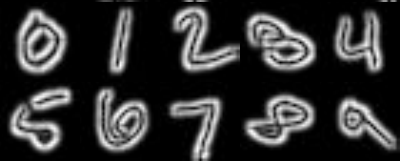
\includegraphics[width=0.4\textwidth]{figures/rotacion}} \hspace{10pt}
	\subfigure[]{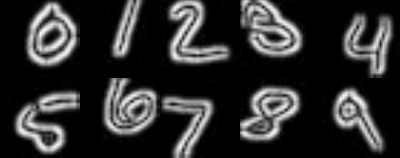
\includegraphics[width=0.4\textwidth]{figures/traslacion}} \hspace{10pt}
	\subfigure[]{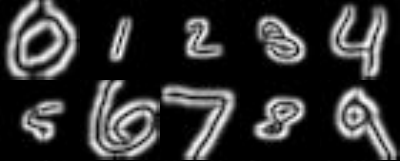
\includegraphics[width=0.4\textwidth]{figures/escala}} \hspace{10pt}
	\subfigure[]{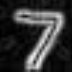
\includegraphics[width=0.4\textwidth]{figures/ruido}}
	\caption{Muestras de imágenes transformadas: (a)~rotación, (b)~traslación, (c)~escalado, (d)~contaminación con ruido aditivo.}
	\label{fig.transformaciones}
\end{figure}

\subsection{Aprendizaje con bases de datos aumentadas} \label{sec.transformaciones}
Para evaluar el efecto que tienen las transformaciones anteriores se genera una base de datos de test para cada transformación, a partir de la que proporciona \acrshort{mnist} de 10000 muestras. En estas nuevas bases de datos se incluyen 6 imágenes con la transformación aplicada para cada uno de los ejemplos y la imagen original. Por último, se aplica el filtro de Sobel a cada uno de los ejemplos, obteniendo una base de datos de test con 70000 ejemplos para cada una de las transformaciones. Estas nuevas bases de datos serán presentadas a la misma red neuronal, diseñada para trabajar sobre imágenes con bordes de Sobel, para poder evaluar la robustez de la misma.\\

Además de las bases de datos creadas mediante la aplicación de una única transformación, se elabora una nueva base de datos que contiene una combinación de todas las transformaciones: escalado, traslación, rotación y contaminación con ruido, para obtener una evaluación más realista. En esta combinación, a la hora de aplicar la traslación, se tendrá en cuenta el factor de escala aplicado, de tal manera que si es mayor que 1, es decir, la imagen se ha ampliado, el rango de desplazamiento se ve reducido a la mitad en ambas direcciones. De esta manera, el dígito se mantendrá siempre dentro de la imagen, sin verse recortado por ningún lado.\\

En la Figura~\ref{fig.mix} se muestra la aplicación de la traslación para cada dígito mostrado en la Figura~\ref{fig.digitosMNIST}.
\begin{figure}[H]
	\begin{center}
		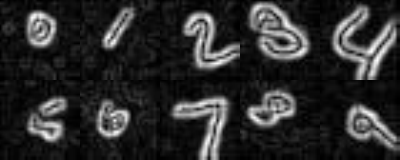
\includegraphics[width=0.4\textwidth]{figures/mix}
		\caption{Muestra de dígitos con mezcla de transformaciones.}
		\label{fig.mix}
	\end{center}
\end{figure}

Una vez obtenidas las nuevas bases de datos, se incluirán en el banco de pruebas de la Sección~\ref{sec.banco} y se obtendrá la tasa de acierto, desglosada por dígitos y de manera global. Estos resultados quedan reflejados en la Figura~\ref{fig.sobelEval}.

\begin{figure}[H]
	\begin{center}
		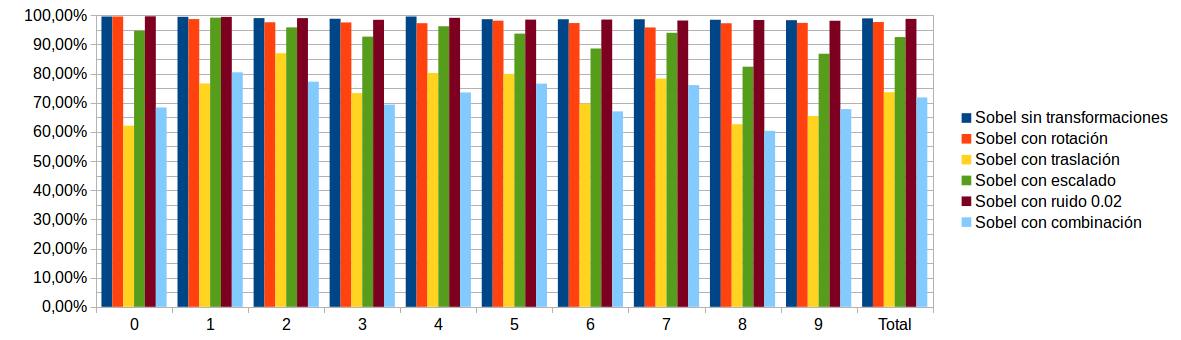
\includegraphics[width=1\textwidth]{figures/sobelev}
		\caption{\textit{Accuracy} para cada dígito y global en la red entrenada con imágenes de bordes Sobel evaluada con bases de datos transformadas.}
		\label{fig.sobelEval}
	\end{center}
\end{figure}

Se observa que el hecho de introducir varias transformaciones sobre la imagen hace que la tasa de acierto disminuya considerablemente, siendo especialmente sensible a la traslación, mientras que el ruido apenas afecta, algo que concuerda con las imágenes mostradas. Estos resultados hacen ver que la red, en un escenario real no reaccionaría de la manera que se desearía, existiendo una probabilidad de fallo del 0.3 si se consideran la combinación de las transformaciones.\\

Para desarrollar una red más robusta se elabora una nueva base de datos de entrenamiento/validación mediante la combinación de las transformaciones explicadas anteriormente. La nueva base de datos será una modificación de la utilizada en la red básica, presentada en la Sección~\ref{sec.red}. Para la evaluación de todas las redes creadas se empleará la base de datos de test que combina todas las transformaciones, con 70000 muestras.\\

En primer lugar, se calcula la matriz de confusión de la red entrenada únicamente con las imágenes de bordes de Sobel utilizando la base de datos de test ampliada con la combinación de transformaciones, que queda reflejada en la Tabla~\ref{tab.matriz1-0}. De esta manera se podrán obtener valores de \textit{precision} y \textit{recall}  y hacer una comparación adecuada de todas las redes.\\
\begin{table}[H]
	\centering
	\begin{tabular}{|c|l|c|c|c|c|c|c|c|c|c|c|c|}
		\cline{3-13} 
		\multicolumn{2}{c|}{} & \multicolumn{11}{c|}{\textbf{Real}} \\ \cline{3-13} 
		\multicolumn{2}{c|}{} & \textbf{0} & \textbf{1} & \textbf{2} &  \textbf{3} & \textbf{4} & \textbf{5} & \textbf{6} & \textbf{7} & \textbf{8} & \textbf{9} & \textbf{Total}\\ \hline
		\multirow{10}{0.5cm}{\rotatebox{90}{\textbf{Predicción}}}& \textbf{0} &  \cellcolor{lightgray}4691 & 191 & 82 & 90 & 118 & 83 & 173 & 45 & 163 & 192 & 5828\\ \cline{2-13}
		& \textbf{1} & 76 & \cellcolor{lightgray}6391 & 119 & 65 & 213 & 22 & 209 & 212 & 246 & 142 & 7695\\ \cline{2-13}
		& \textbf{2} & 188 & 98 & \cellcolor{lightgray}5578 & 462 & 232 & 131 & 121 & 683 & 276 & 229 & 7998\\ \cline{2-13}
		& \textbf{3} & 43 & 30 & 443 & \cellcolor{lightgray}4904 & 270 & 201 & 48 & 275 & 243 & 311 & 6768\\ \cline{2-13}
		& \textbf{4} & 158 & 415 & 291 & 145 & \cellcolor{lightgray}5055 & 117 & 720 & 37 & 320 & 381 & 7639\\ \cline{2-13}
		& \textbf{5} & 96 & 72 & 65 & 633 & 107 & \cellcolor{lightgray}4780 & 234 & 112 & 323 & 243 & 6665\\ \cline{2-13}
		& \textbf{6} & 472 & 234 & 86 & 49 & 130 & 216 & \cellcolor{lightgray}4497 & 15 & 326 & 91 & 6116\\ \cline{2-13}
		& \textbf{7} & 57 & 416 & 265 & 255 & 244 & 105 & 19 & \cellcolor{lightgray}5473 & 235 & 488 & 7557\\ \cline{2-13}
		& \textbf{8} & 138 & 80 & 131 & 139 & 139 & 129 & 182 & 84 & \cellcolor{lightgray}4116 & 194 & 5332\\ \cline{2-13}
		& \textbf{9} & 941 & 18 & 164 & 328 & 366 & 460 & 503 & 260 & 570 & \cellcolor{lightgray}4792 & 8402\\ \cline{2-13} 
		& \textbf{Total} & 6860 & 7945 & 7224 & 7070 & 6874 & 6244 & 6706 & 7196 & 6818 & 7063 & 70000\\ \hline
	\end{tabular}
	\caption{Matriz de confusión red 1-0 sobre base de datos de test ampliada con combinación de transformaciones.}
	\label{tab.matriz1-0}
\end{table}

Tras obtener la evaluación de la red básica, se procede a su modificación y posterior evaluación, variando el número de imágenes transformadas que se utilizan, así como la inclusión o no de la imagen original. Para esta tarea se parte de la base de datos de entrenamiento, modificada de la misma manera que se modificó la de test en la sección anterior, obteniendo 6 transformaciones y la imagen original. Tras evaluar los resultados se irá reduciendo el número de imágenes incluidas en la base de datos de entrenamiento, para evaluar el impacto y conseguir una base de datos que proporcione buenos resultados disminuyendo la complejidad de cómputo.
\vspace{5pt}

\begin{description}
	\item[Base de datos 1-6] \hfill 
	\vspace{5pt}
	\\
	Para elaborar esta base de datos se utilizan 6 imágenes transformadas y la imagen original, todas ellas con la aplicación de los filtros de Sobel. De esta forma se obtiene una base de datos de entrenamiento de 336000 muestras y una de validación de 84000 muestras.\\
	\vspace{-10pt}
	\\
	Con estas bases de datos se entrena una nueva red y se calcula la matriz de confusión utilizando la base de datos de test ampliada con combinación de transformaciones, mostrada en la Tabla~\ref{tab.matriz1-6}.
	\begin{table}[H]
		\centering
		\begin{tabular}{|c|l|c|c|c|c|c|c|c|c|c|c|c|}
			\cline{3-13}  
			\multicolumn{2}{c|}{} & \multicolumn{11}{c|}{\textbf{Real}} \\ \cline{3-13} 
			\multicolumn{2}{c|}{} & \textbf{0} & \textbf{1} & \textbf{2} &  \textbf{3} & \textbf{4} & \textbf{5} & \textbf{6} & \textbf{7} & \textbf{8} & \textbf{9} & \textbf{Total}\\ \hline
			\multirow{10}{0.5cm}{\rotatebox{90}{\textbf{Predicción}}}& \textbf{0} & \cellcolor{lightgray}6770 & 13 & 24 & 13 & 7 & 35 & 74 & 2 & 161 & 40 & 7139\\ \cline{2-13}
			& \textbf{1} & 1 & \cellcolor{lightgray}7868 & 26 & 15 & 13 & 15 & 25 & 43 & 11 & 12 & 8029\\ \cline{2-13}
			& \textbf{2} & 13 & 16 & \cellcolor{lightgray}6890 & 125 & 5 & 10 & 6 & 62 & 47 & 8 & 7182\\ \cline{2-13}
			& \textbf{3} & 1 & 3 & 9 & \cellcolor{lightgray}6567 & 0 & 66 & 0 & 3 & 9 & 8 & 6666\\ \cline{2-13}
			& \textbf{4} & 18 & 3 & 53 & 13 & \cellcolor{lightgray}6610 & 24 & 52 & 9 & 74 & 71 & 6927\\ \cline{2-13}
			& \textbf{5} & 3 & 0 & 1 & 95 & 0 & \cellcolor{lightgray}5820 & 16 & 2 & 17 & 5 &5959\\ \cline{2-13}
			& \textbf{6} & 25 & 10 & 7 & 3 & 10 & 123 & \cellcolor{lightgray}6519 & 0 & 71 & 2 & 6770\\ \cline{2-13}
			& \textbf{7} & 13 & 25 & 170 & 119 & 32 & 17 & 1 & \cellcolor{lightgray}7030 & 43 & 108 & 7558\\ \cline{2-13}
			& \textbf{8} & 4 & 7 & 31 & 54 & 7 & 67 & 9 & 8 & \cellcolor{lightgray}6234 & 12 & 6433\\ \cline{2-13}
			& \textbf{9} & 12 & 0 & 13 & 66 & 190 & 67 & 4 & 37 & 151 & \cellcolor{lightgray}6797 & 7337\\ \cline{2-13}
			& \textbf{Total} & 6860 & 7945 & 7224 & 7070 & 6874 & 6244 & 6706 & 7196 & 6818 & 7063 & 70000\\ \hline
		\end{tabular}
		\caption{Matriz de confusión red 1-6 sobre base de datos de test ampliada con combinación de transformaciones.}
		\label{tab.matriz1-6}
	\end{table}
	\item[Base de datos 1-1] \hfill 
	\vspace{5pt}
	\\
	En este caso se reducirá el número de imágenes transformadas para comprobar la importancia de las mismas en el aprendizaje. El objetivo es tratar de reducir el número de muestras en la base de datos de entrenamiento y validación para disminuir la carga computacional manteniendo las prestaciones.\\
	\vspace{-10pt}
	\\
	Para lograr el objetivo se incluirá en la base de datos de entrenamiento y de validación una única imagen transformada y la imagen original, obteniendo un total de 96000 muestras en la base de datos de entrenamiento y 24000 en la de validación.\\
	\vspace{-10pt}
	\\
	Tras obtener las bases de datos se entrenará una nueva red de la que se obtendrá de nuevo la matriz de confusión utilizando la base de datos de test ampliada con combinación de transformaciones, representada en la Tabla~\ref{tab.matriz1-1}.
	\begin{table}[H]
		\centering
		\begin{tabular}{|c|l|c|c|c|c|c|c|c|c|c|c|c|}
			\cline{3-13} 
			\multicolumn{2}{c|}{} & \multicolumn{11}{c|}{\textbf{Real}} \\ \cline{3-13} 
			\multicolumn{2}{c|}{} & \textbf{0} & \textbf{1} & \textbf{2} &  \textbf{3} & \textbf{4} & \textbf{5} & \textbf{6} & \textbf{7} & \textbf{8} & \textbf{9} & \textbf{Total}\\ \hline
			\multirow{10}{0.5cm}{\rotatebox{90}{\textbf{Predicción}}}& \textbf{0} & \cellcolor{lightgray}6637 & 6 & 29 & 8 & 9 & 11 & 36 & 4 & 56 & 39 & 6835\\ \cline{2-13}
			& \textbf{1} & 3 & \cellcolor{lightgray}7821 & 29 & 9 & 16 & 4 & 18 & 35 & 5 & 16 & 7956\\ \cline{2-13}
			& \textbf{2} & 13 & 10 & \cellcolor{lightgray}6747 & 45 & 21 & 2 & 8 & 107 & 37 & 12 & 7002\\ \cline{2-13}
			& \textbf{3} & 8 & 16 & 117 & \cellcolor{lightgray}6703 & 2 & 97 & 4 & 35 & 66 & 42 & 7090\\ \cline{2-13}
			& \textbf{4} & 2 & 4 & 45 & 10 & \cellcolor{lightgray}6576 & 9 & 41 & 33 & 38 & 164 & 6922\\ \cline{2-13}
			& \textbf{5} & 26 & 4 & 27 & 152 & 18 & \cellcolor{lightgray}5989 & 80 & 28 & 84 & 91 & 6499\\ \cline{2-13}
			& \textbf{6} & 116 & 31 & 10 & 2 & 66 & 51 & \cellcolor{lightgray}6474 & 0 & 82 & 10 & 6842\\ \cline{2-13}
			& \textbf{7} & 19 & 30 & 135 & 58 & 29 & 12 & 0 & \cellcolor{lightgray}6873 & 27 & 89 & 7272\\ \cline{2-13}
			& \textbf{8} & 23 & 21 & 68 & 70 & 35 & 54 & 41 & 20 & \cellcolor{lightgray}6345 & 66 & 6743\\ \cline{2-13}
			& \textbf{9} & 13 & 2 & 17 & 13 & 102 & 15 & 4 & 61 & 78 & \cellcolor{lightgray}6534 & 6839\\ \cline{2-13}
			& \textbf{Total} & 6860 & 7945 & 7224 & 7070 & 6874 & 6244 & 6706 & 7196 & 6818 & 7063 & 70000\\ \hline
		\end{tabular}
		\caption{Matriz de confusión red 1-1 sobre base de datos de test ampliada con combinación de transformaciones.}
		\label{tab.matriz1-1}
	\end{table}
	\item[Base de datos 0-6] \hfill 
	\vspace{10pt}
	\\
	Esta reducción consiste en mantener las 6 transformaciones de la imagen en cada muestra, pero no incluir la original. De esta manera se podrá establecer una conclusión sobre la importancia de la imagen original en el aprendizaje.\\
	\vspace{-10pt}
	\\
	En esta ocasión se tendrá una base de datos de entrenamiento con 288000 muestras y una de validación con 72000. Al igual que en los casos anteriores se entrenará una nueva red y se obtendrá su matriz de confusión utilizando la base de datos de test ampliada con combinación de transformaciones, respresentada en la Tabla~\ref{tab.matriz0-6}.
	\begin{table}[H]
		\centering
		\begin{tabular}{|c|l|c|c|c|c|c|c|c|c|c|c|c|}
			\cline{3-13} 
			\multicolumn{2}{c|}{} & \multicolumn{11}{c|}{\textbf{Real}} \\ \cline{3-13} 
			\multicolumn{2}{c|}{} & \textbf{0} & \textbf{1} & \textbf{2} &  \textbf{3} & \textbf{4} & \textbf{5} & \textbf{6} & \textbf{7} & \textbf{8} & \textbf{9} & \textbf{Total}\\ \hline
			\multirow{10}{0.5cm}{\rotatebox{90}{\textbf{Predicción}}}& \textbf{0} & \cellcolor{lightgray}6639 & 0 & 23 & 8 & 5 & 12 & 16 & 1 & 41 & 16 & 6761\\ \cline{2-13}
			& \textbf{1} & 4 & \cellcolor{lightgray}7853 & 12 & 8 & 14 & 1 & 11 & 62 & 2 & 13 & 7980\\ \cline{2-13}
			& \textbf{2} & 14 & 18 & \cellcolor{lightgray}7022 & 78 & 31 & 6 & 13 & 133 & 58 & 6 & 7379\\ \cline{2-13}
			& \textbf{3} & 1 & 15 & 29 & \cellcolor{lightgray}6797 & 1 & 69 & 4 & 29 & 32 & 27 & 7004\\ \cline{2-13}
			& \textbf{4} & 12 & 5 & 21 & 1 & \cellcolor{lightgray}6675 & 3 & 24 & 24 & 40 & 149 & 6954\\ \cline{2-13}
			& \textbf{5} & 19 & 3 & 4 & 90 & 7 & \cellcolor{lightgray}6065 & 57 & 7 & 91 & 50 & 6393\\ \cline{2-13}
			& \textbf{6} & 117 & 23 & 9 & 1 & 19 & 46 & \cellcolor{lightgray}6545 & 0 & 62 & 7 & 6829\\ \cline{2-13}
			& \textbf{7} & 16 & 13 & 58 & 43 & 12 & 6 & 0 & \cellcolor{lightgray}6859 & 24 & 65 & 7096\\ \cline{2-13}
			& \textbf{8} & 30 & 13 & 36 & 34 & 15 & 27 & 36 & 10 & \cellcolor{lightgray}6399 & 30 & 6630\\ \cline{2-13}
			& \textbf{9} & 8 & 2 & 10 & 10 & 95 & 9 & 0 & 71 & 69 & \cellcolor{lightgray}6700 & 6974\\ \cline{2-13}
			& \textbf{Total} & 6860 & 7945 & 7224 & 7070 & 6874 & 6244 & 6706 & 7196 & 6818 & 7063 & 70000\\ \hline
		\end{tabular}
		\caption{Matriz de confusión red 0-6 sobre base de datos de test ampliada con combinación de transformaciones.}
		\label{tab.matriz0-6}
	\end{table}
	\item[Base de datos 0-1] \hfill 
	\vspace{10pt}
	\\
	Finalmente, puesto que los resultados de la reducción de muestras en el entrenamiento resultan bastante satisfactorios, se reduce el número de imágenes transformadas y no se incluye la imagen original, obteniendo una base de datos de entrenamiento de 48000 muestras y de validación de 12000.\\
	\vspace{-10pt}
	\\
	Con esta nueva base de datos se entrena una nueva red y se obtiene su matriz de confusión utilizando la base de datos de test ampliada con combinación de transformaciones, reflejada en la Tabla~\ref{tab.matriz0-1}.
	\begin{table}[H]
		\centering
		\begin{tabular}{|c|l|c|c|c|c|c|c|c|c|c|c|c|}
			\cline{3-13} 
			\multicolumn{2}{c|}{} & \multicolumn{11}{c|}{\textbf{Real}} \\ \cline{3-13} 
			\multicolumn{2}{c|}{} & \textbf{0} & \textbf{1} & \textbf{2} &  \textbf{3} & \textbf{4} & \textbf{5} & \textbf{6} & \textbf{7} & \textbf{8} & \textbf{9} & \textbf{Total}\\ \hline
			\multirow{10}{0.5cm}{\rotatebox{90}{\textbf{Predicción}}}& \textbf{0} & \cellcolor{lightgray}6728 & 4 & 31 & 10 & 11 & 18 & 63 & 6 & 66 & 41 & 6978\\ \cline{2-13}
			& \textbf{1} & 2 & \cellcolor{lightgray}7854 & 32 & 8 & 26 & 7 & 27 & 72 & 9 & 20 & 8057\\ \cline{2-13}
			& \textbf{2} & 10 & 22 & \cellcolor{lightgray}6873 & 79 & 27 & 11 & 15 & 145 & 59 & 13 & 7254\\ \cline{2-13}
			& \textbf{3} & 5 & 15 & 51 & \cellcolor{lightgray}6661 & 6 & 79 & 5 & 38 & 30 & 27 & 6917\\ \cline{2-13}
			& \textbf{4} & 1 & 2 & 39 & 6 & \cellcolor{lightgray}6348 & 2 & 25 & 16 & 31 & 65 & 6535\\ \cline{2-13}
			& \textbf{5} & 15 & 1 & 7 & 137 & 6 & \cellcolor{lightgray}5964 & 64 & 11 & 61 & 43 & 6309\\ \cline{2-13}
			& \textbf{6} & 45 & 16 & 12 & 3 & 38 & 61 & \cellcolor{lightgray}6462 & 0 & 60 & 8 & 6705\\ \cline{2-13}
			& \textbf{7} & 14 & 18 & 93 & 55 & 33 & 10 & 0 & \cellcolor{lightgray}6833 & 25 & 86 & 7167\\ \cline{2-13}
			& \textbf{8} & 26 & 12 & 73 & 88 & 62 & 56 & 40 & 12 & \cellcolor{lightgray}6391 & 52 & 6812\\ \cline{2-13}
			& \textbf{9} & 14 & 1 & 13 & 23 & 317 & 36 & 5 & 63 & 86 & \cellcolor{lightgray}6708 & 7266\\ \cline{2-13}
			& \textbf{Total} & 6860 & 7945 & 7224 & 7070 & 6874 & 6244 & 6706 & 7196 & 6818 & 7063 & 70000\\ \hline
		\end{tabular}
		\caption{Matriz de confusión red 0-1 sobre base de datos de test ampliada con combinación de transformaciones.}
		\label{tab.matriz0-1}
	\end{table}
\end{description}

Una vez obtenidas las matrices de confusión de cada red neuronal entrenada, se pueden establecer algunas conclusiones a simple vista. En primer lugar, es clara la mejora al entrenar introduciendo alguna imagen ruidosa: si se observan los valores de la diagonal, correspondiente con los dígitos correctamente clasificados, estos valores son superiores al introducir ruido en el entrenamiento. Además, entrenar introduciendo un mayor número de imágenes ruidosas, aparentemente, no aporta gran información a la red, siendo los resultados muy similares en las redes 1-6 y 1-1. Finalmente, introducir la imagen original en el entrenamiento tampoco aporta información fundamental, pues los resultados obtenidos con la red 1-1 y la red 0-1 son muy similares, al igual que ocurre con las redes 1-6 y 0-6.\\

Para establecer conclusiones más firmes, se calculan el \textit{precision} y \textit{recall} de cada una de las redes. Estos resultados quedan reflejados en la Figura~\ref{fig.precision-recall} que confirman las conclusiones alcanzadas con anterioridad: (1) Existe una clara mejora al introducir imágenes ruidosas en el entrenamiento; (2) una única imagen ruidosa aporta suficiente información; y (3) la inclusión de la imagen original no aporta gran información para el entrenamiento.\\
\begin{figure}[H]
	\centering
	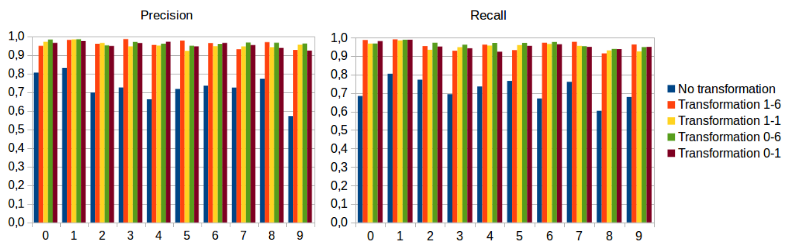
\includegraphics[width=0.9\textwidth]{figures/precision-recall}
	\caption{Resultados de \textit{Precision} y \textit{Recall} para la red entrenada con imágenes de bordes y las redes entrenadas con transformaciones (1-6,1-1,0-6,0-1), sobre base de datos de test ampliada con combinación de transformaciones}
	\label{fig.precision-recall}
\end{figure}


Tras mejorar la red en cuanto a términos de precisión con el cambio en las bases de datos, se analizará la posibilidad de reducir el número de iteraciones para disminuir la carga de cómputo en el entrenamiento de la red.

\subsection{Número de iteraciones}
Hasta ahora, se había fijado el número de iteraciones en el entrenamiento de la red en un valor de 10000, siendo la iteración, según lo explicado en la Sección~\ref{sec.caffe}, el paso de un \textit{batch}. Sin embargo, este número de iteraciones no tiene por qué ser el más idóneo para la aplicación.\\

Durante el entrenamiento de una red neuronal, el aprendizaje es progresivo. De esta manera es previsible que la red obtenida en la iteración \textit{n+1} sea mejor que la obtenida en la iteración \textit{n}. Existe un momento durante el entrenamiento de la red en el que la mejora entre iteraciones consecutivas es prácticamente nula, pudiéndose producir, incluso, un deterioro en las prestaciones de red. Este deterioro es conocido como sobreaprendizaje, producido por la excesiva focalización en las muestras proporcionadas en el entrenamiento, empeorando la generalización.\\
\vspace{10pt}

Como se comentó en la Sección~\ref{sec.red}, Caffe permite obtener durante el entrenamiento un archivo \textit{log} donde se plasman los datos de \textit{accuracy} calculados cada cierto número de iteraciones. Estos resultados han sido recogidos para cada una de las redes explicadas en la sección anterior, obteniendo una comparativa, mostrada en la Figura~\ref{fig.iteraciones}, que permita seleccionar la red más adecuada para la aplicación.
\begin{figure}[H]
	\begin{center}
		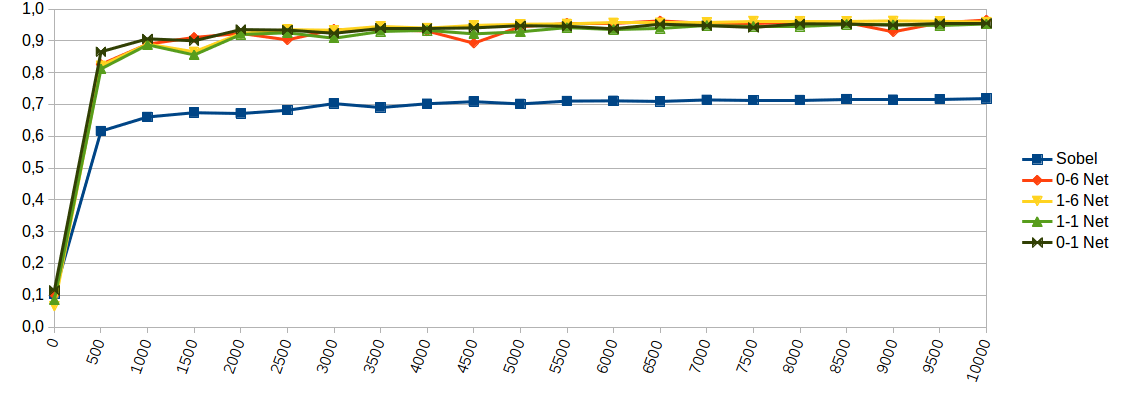
\includegraphics[width=0.8\textwidth]{figures/iteraciones}
		\caption{Valores de \textit{Accuracy} en redes intermedias para cada una de las redes entrenadas.}
		\label{fig.iteraciones}
	\end{center}
\end{figure}
En la Figura~\ref{fig.iteraciones} se puede comprobar que, además de la mejora mencionada anteriormente al introducir imágenes ruidosas en el entrenamiento, la estabilidad de la red se alcanza mucho antes de las 10000 iteraciones marcadas.\\

Por todo lo mencionado anteriormente, se decide escoger la red entrenada con la base de datos 0-1, parando el entrenamiento en la iteración 5000. De esta manera, se disminuye consideráblemente la carga computacional, ya que se reduce más de la mitad el número de iteraciones de entrenamiento de la red y se mantiene el número de muestras de entrenamiento y validación, manteniendo una buena capacidad de generalización.

\section{Experimentos}
Tras el análisis realizado anteriormente se ha obtenido una red neuronal más robusta, que permite una mejor clasificación en tiempo real de los dígitos mostrados a la cámara. Con todo lo estudiado en puntos anteriores se realiza una comparación entre la primera red básica que se desarrolló y la red escogida tras el estudio de los efectos del aprendizaje, realizado en la Sección~\ref{sec.aprendizaje}.\\

En primer lugar se prueba la aplicación con una imagen sintética, donde el dígito se obtuvo con el ordenador y el fondo es negro, tal y como se entrenó la primera red desarrollada. Los resultados de este experimento quedan reflejados en la Figura~\ref{fig.experimento1}.

\begin{figure}[H]
	\centering
	\subfigure[]{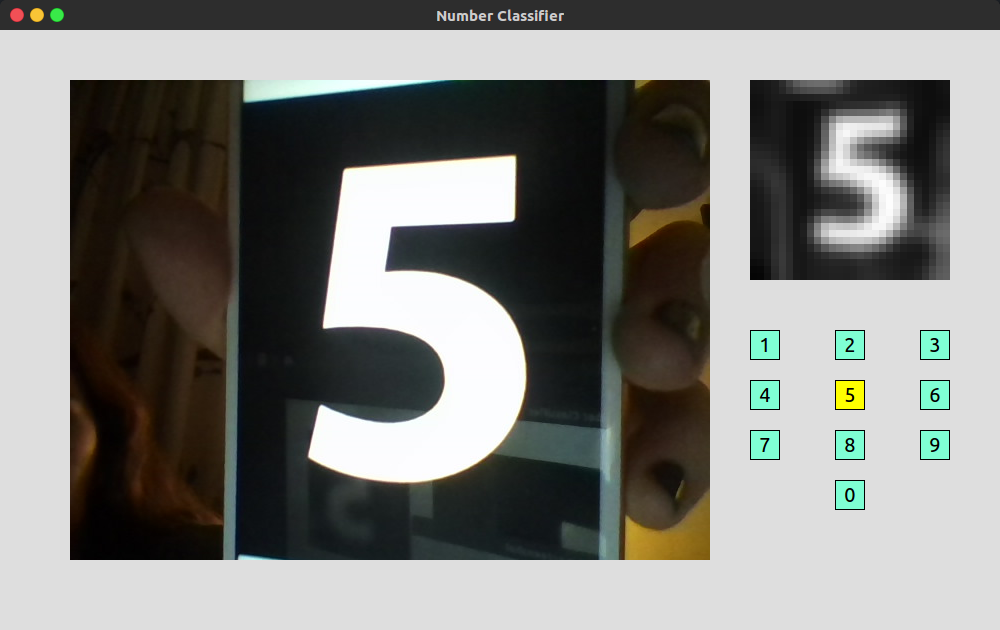
\includegraphics[width=0.4\textwidth]{figures/exp_basica1}} \hspace{5pt}
	\subfigure[]{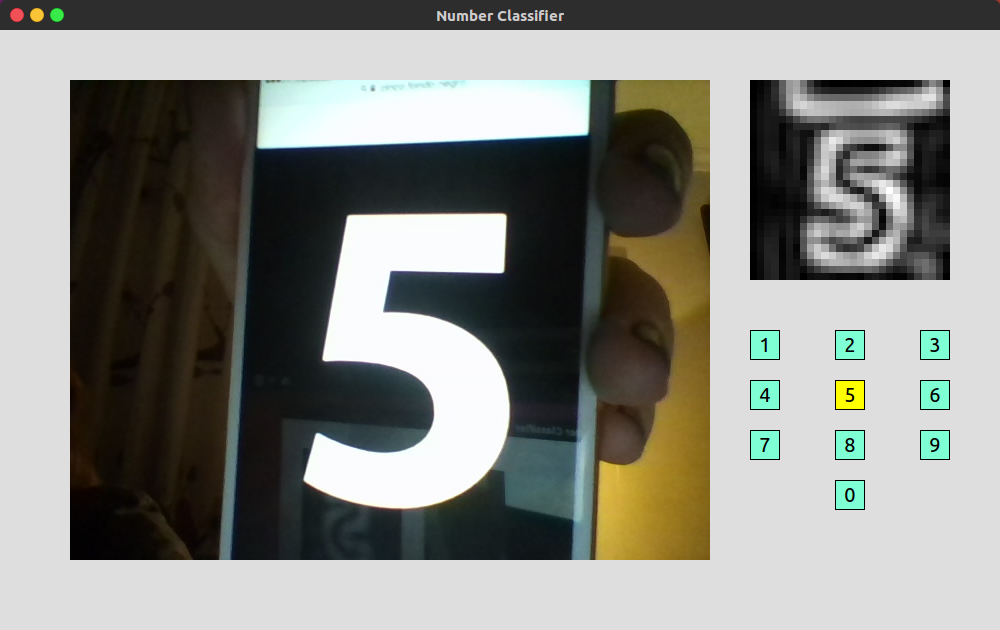
\includegraphics[width=0.4\textwidth]{figures/exp_robusta1}}
	\caption{Evaluación de la aplicación con dígito sintético: (a)~red básica, (b)~red robusta.}
	\label{fig.experimento1}
\end{figure}

Tras evaluar un ejemplo sintético se pone a prueba la aplicación con una imagen más complicada, variando el fondo y escribiéndolo a mano. En la Figura~\ref{fig.experimento}, se comprueba cómo un dígito que no lograba ser identificado con la red básica, sí lo hace con la red más robusta obtenida tras el estudio. 

\begin{figure}[H]
	\centering
	\subfigure[]{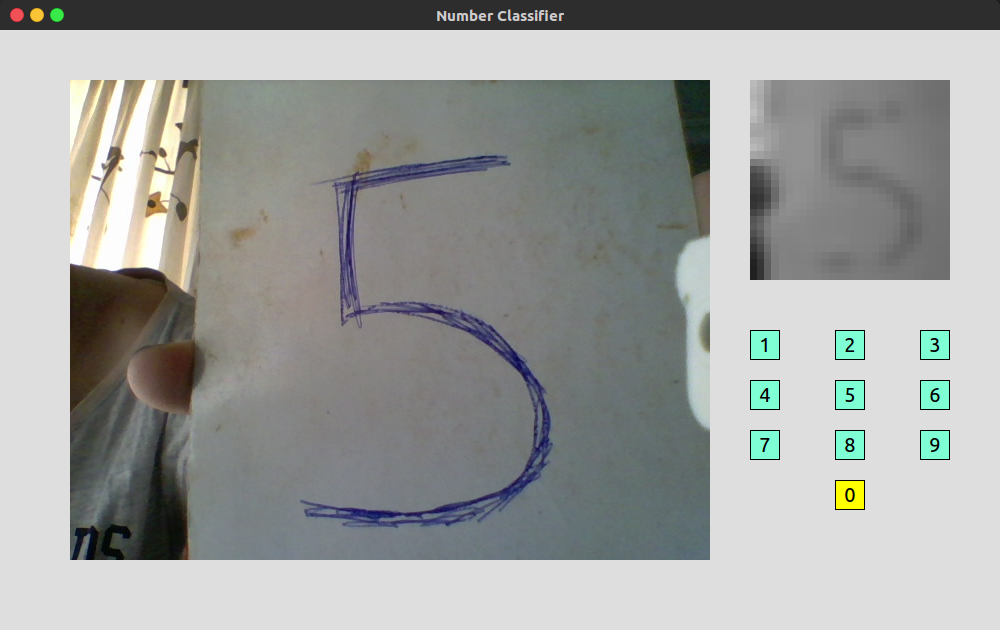
\includegraphics[width=0.4\textwidth]{figures/exp_basica}} \hspace{5pt}
	\subfigure[]{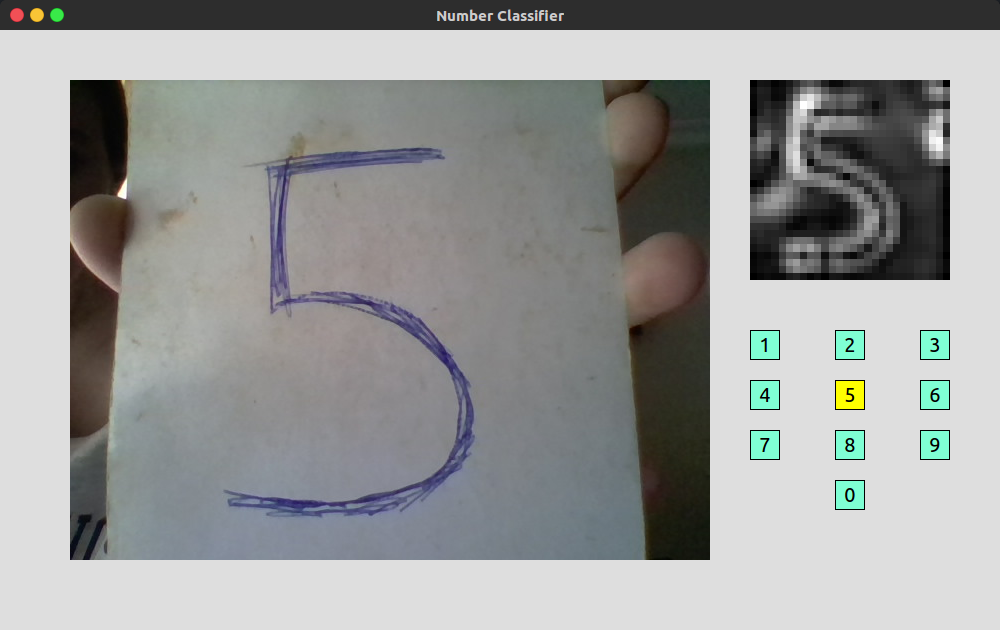
\includegraphics[width=0.4\textwidth]{figures/exp_robusta}}
	\caption{Evaluación de la aplicación con dígito manuscrito sobre fondo blanco: (a)~red básica, (b)~red robusta.}
	\label{fig.experimento}
\end{figure}
\vspace{20pt}

Para realizar los experimentos anteriores se ha tomado como red básica, la presentada en la Sección~\ref{sec.red}, en cuyo entrenamiento únicamente se disponía de imágenes con fondo negro y el dígito aparece en blanco. Como era de esperar, al mostrar a la cámara un dígito con el fondo blanco la red hace una clasificación errónea. En el caso de la red robusta, se ha seleccionado la red que se concluyó tras la Sección~\ref{sec.aprendizaje}, entrenada con imágenes transformadas a las que se les ha aplicado el filtro de bordes Sobel. Esta red permite independizar la imagen del fondo y que la imagen obtenida por la cámara no sea tan perfecta. Con esta nueva red la aplicación sí consigue clasificar correctamente el dígito mostrado a la cámara.\\

La aplicación desarrollada es una muestra sencilla de herramienta para la clasificación de imágenes mediante técnicas de aprendizaje profundo. Este ejemplo abre una nueva puerta para abarcar nuevos problemas de clasificación más complejos, con bases de datos más completas, que permitan solucionar problemas de interés para el ser humano.
